\chapter{A Distributed NSB Algorithm for Formation Path Following}
\label{chap:distr_NSB}

This chapter presents a distributed null-space-based behavioral algorithm for the formation path-following problem of vehicles moving in three dimensions.
The algorithm is applied to fleets of underactuated autonomous underwater vehicles.
The algorithm combines null-space-based control with consensus methods.
First, we present a continuous-time version of the algorithm and prove its stability using Lyapunov analysis.
Then, we present a discrete-time event-triggered version that, compared to similar formation path-following methods, can achieve the same steady state-error performance with fewer inter-vehicle transmissions.
The effectiveness of both the continuous-time and the discrete-time algorithm is verified in numerical simulations.
Furthermore, the discrete-time version is tested in field experiments.  
The contents of this chaper are based on \cite{matous_singularity_2023}.

The chapter is organized as follows.
Section~\ref{sec:distr_NSB_problem} defines the formation path following problem.
Section~\ref{sec:distr_NSB_NSB} presents the centralized \gls{nsb} algorithm.
In Section~\ref{sec:distr_NSB_distributed_NSB}, we present the continuous-time distributed \gls{nsb} algorithm, and in Section~\ref{sec:distr_NSB_closed_loop}, we analyze its closed-loop behavior.
Section~\ref{sec:distr_NSB_AUV} discusses how to apply the proposed algorithm to underactuated \glspl{auv} and proposes the discrete-time modification.
Finally, Sections~\ref{sec:distr_NSB_simulations} and \ref{sec:distr_NSB_experiments} present the results of numerical simulations and experiments, respectively.

\section{Problem Definition}
\label{sec:distr_NSB_problem}
We begin by considering a group of $N$ vehicles with single-integrator dynamics.
An extension to more complex vehicle models will be shown in Section~\ref{sec:distr_NSB_AUV}.
Let $\mat{p}_i \in \mathbb{R}^3$ be the position of vehicle $i$.
The kinematic equation of vehicle $i$ is
\begin{equation}
    \dot{\mat{p}}_i = \ivel_i,
    \label{eq:distr_NSB_kinematics}
\end{equation}
where $\ivel_i \in \mathbb{R}^3$ is the input velocity.

The vehicles should follow a predefined path in a given formation.
Let $\mat{p}_p: \mathbb{R} \mapsto \mathbb{R}^3$ be a parametrization of the desired path.
We assume that the function is $\mathcal{C}^1$ and regular.
Consequently, for any point $\mat{p}_p(s)$, there exists a path-tangential coordinate frame and a corresponding rotation matrix $\mat{R}_p(s)$.

The path-following error $\mat{p}_b^p$ is given by the position of the barycenter in the path-tangential coordinate frame 
\begin{align}
    \mat{p}_b^p &= \mat{R}_p\T \, \big(\mat{p}_b - \mat{p}_p(s)\big), &
    \mat{p}_b &= \frac{1}{n} \sum_{i=1}^n \mat{p}_i.
    \label{eq:distr_NSB_barycenter}
\end{align}
The goal of path following is to control the vehicles so that $\mat{p}_b^p \rightarrow \mat{0}_3$.

The vehicles should converge to a dynamic formation that rotates with the desired path (see Section~\ref{sec:background_formation_keeping} for details).
Let $\mat{p}_{f,1}^f, \ldots, \mat{p}_{f,n}^f$ be the position vectors that represent the desired formation.
The objective is to control the vehicles so that
\begin{align}
    \mat{p}_i - \mat{p}_b &\rightarrow \mat{R}_p(s) \mat{p}_{f,i}^f + \mat{p}_b, &
    i &\in \left\{1, \ldots, n \right\}.
\end{align}

\section{NSB Algorithm for the Formation Path Following Problem}
\label{sec:distr_NSB_NSB}
In this section, we present the centralized formation path-following \gls{nsb} algorithm for vehicles moving in three dimensions.
The algorithm is a simplified version of the two methods presented in Chapters~\ref{chap:5dof_nsb} and \ref{chap:NSB_R}.

For the sake of simplicity, we do not consider inter-vehicle collision avoidance.
Instead, we focus on the formation path-following problem with obstacle avoidance.
To solve the problem, we define two tasks: path following and formation keeping.
Obstacle avoidance is not implemented as a separate task but rather as an extension of path-following.

In the \emph{nominal} case (\emph{i.e.,} when obstacle avoidance is not active), the path-following velocity is given by the coupled \acrfull{los} guidance law \eqref{eq:background_los_coupled}
\begin{align}
    \ivel_{\rm LOS} &= \frac{U_d}{D} \mat{R}_p \inlinevector{\Delta, -y_b^p, -z_b^p}, &
    D &= \norm{\inlinevector{\Delta, -y_b^p, -z_b^p}},
    \label{eq:distr_NSB_v_LOS_centralized}
\end{align}
with a constant lookahead distance $\Delta > 0$.

The method for obstacle avoidance is identical to the one presented in Chapter~\ref{chap:NSB_R}.
Let $\mat{p}_o \in \mathbb{R}^2$ and $\ivel_o \in \mathbb{R}^2$ denote the position and velocity of the obstacle.
When the task is active, the $x$- and $y$-components of the LOS velocity are replaced by the obstacle avoidance velocity $\ivel_{\rm OA}$ given by
\begin{align}
    \ivel_{\rm OA} &= \norm{\ivel_{\rm rel}} \inlinevector{\cos(\psi_{\rm OA}), \sin(\psi_{\rm OA})} + \inlinevector{\dot{x}_o, \dot{y}_o}, \\
    \psi_{\rm OA} &= {\rm arctan}_2 \left(y_o - y_b, x_o - x_b\right) \pm \alpha,
\end{align}
where $\ivel_{\rm rel}$ is the relative velocity and $\alpha$ is the collision cone angle, as defined in \eqref{eq:NSB_R_v_rel} and \eqref{eq:NSB_R_collision-conflict}, respectively.
Note that $\psi_{\rm OA}$ has two solutions corresponding to avoiding the obstacle in the clockwise and counterclockwise directions.
Inspired by \cite{haraldsen_reactive_2021}, we propose the following method for choosing a direction:
When the conflict first happens, we choose the value of $\psi_{\rm OA}$ that is closer to the direction of $\ivel_{\rm rel}$.
Afterwards, we maintain the same direction.

Finally, let us discuss formation keeping.
The proposed formation-keeping law is analogous to \eqref{eq:background_NSB_formation_velocity} and \eqref{eq:nsb_5dof_CLIK}.
The formation-keeping velocity of the whole fleet is given by
\begin{equation}
    \mat{v}_{f} = \mat{J}_f^{\dagger} \left(\dot{\bs{\sigma}}_{d,f} - \bs{\Lambda}_f (\bs{\sigma}_f - \bs{\sigma}_{d,f})\right),
\end{equation}
where $\mat{J}_f$ is the Jacobian of the formation-keeping task, $\bs{\sigma}_f$ is the formation-keeping task variable, and $\bs{\sigma}_{d,f}$ is its desired value, as defined in \eqref{eq:background_NSB_formation_jacobian}, \eqref{eq:background_formation_variable}, and \eqref{eq:background_NSB_formation_reference}, respectively.

Assuming that the gain matrix is chosen as $\bs{\Lambda}_f = k_f \mat{I}$, where $k_f > 0$ is a constant, then the formation-keeping velocity of vehicle $i$ is given by
\begin{align}
    \ivel_{f, i} &= -k_f \left(\bs{\sigma}_i - \bs{\sigma}_{d,i}\right) + \dot{\bs{\sigma}}_{d,i},
    \label{eq:distr_NSB_v_f_centralized}
\end{align}
where 
\begin{align}
    \bs{\sigma}_{i} &= \mat{p}_i - \mat{p}_b, &
    \bs{\sigma}_{d,i} &= \mat{R}_p \mat{p}_{f, i}^f.
\end{align}

Since the formation-keeping and path-following tasks are independent and orthogonal, the total desired \gls{nsb} velocity of vehicle $i$ is given by
\begin{equation}
    \ivel_{{\rm NSB}, i} = \ivel_{\rm LOS} + \ivel_{f, i}.
\end{equation}

Similarly to \eqref{eq:NSB_R_path_update}, we choose the following update law for the path parameter
\begin{equation}
    \dot{s} = U_d \norm{\frac{\partial \mat{p}_p(s)}{\partial s}}^{-1} \left(\frac{\Delta}{D} + k_s f_s\left(x_b^p\right)\right),
    \label{eq:distr_NSB_path_parameter}
\end{equation}
where
\begin{equation}
    f_s(x) = \frac{x}{\sqrt{1 + x}},
\end{equation}
and $k_s$ is a positive gain.

\section{Distributed NSB Algorithm}
\label{sec:distr_NSB_distributed_NSB}
Now, let us discuss how to make the algorithm presented in the previous section distributed.
To perform the \gls{nsb} algorithm in a distributed manner, the vehicles should not need to know the exact positions of each other.
Instead, they should estimate the position of the barycenter and the radius of the formation, and converge to a common value of the path parameter.

Let $\mat{p}_{b, i}$, $r_{f, i}$, and $s_i$ denote vehicle $i$'s estimates of the barycenter, formation radius, and path parameter, respectively.
The vehicle can then calculate its \gls{los} velocity as
\begin{equation}
    \ivel_{{\rm LOS}, i} = \frac{U_d}{D_i} \mat{R}_p(s_i) \inlinevector{\Delta, -y_{b, i}^p, -z_{b, i}^p},
\end{equation}
where
\begin{align}
    \inlinevector{x_{b, i}^p, y_{b, i}^p, z_{b, i}^p} &= \mat{R}_p(s_i)\T \left(\mat{p}_{b, i} - \mat{p}_p\left(s_i\right)\right), \\
    D_i &= \sqrt{\Delta^2 + \left(y_{b, i}^p\right)^2 + \left(z_{b, i}^p\right)^2}.
\end{align}
In addition, the vehicle can estimate the cone angle as
\begin{align}
    \alpha_i &= \arcsin\left(\frac{r_o + r_{f, i}}{\norm{\mat{p}_{{\rm rel}, i}}}\right), &
    \mat{p}_{{\rm rel}, i} &= \mat{p}_o - \inlinevector{x_{b, i}, y_{b, i}},
\end{align}
where $x_{b, i}$ and $y_{b, i}$ are the $x$- and $y$-components of $\mat{p}_{b, i}$.
The vehicle then determines if there is a need for obstacle avoidance according to the rules described in Chapter~\ref{chap:NSB_R}, and calculates its obstacle avoidance velocity as
\begin{align}
    \ivel_{{\rm OA}, i} &= \norm{\ivel_{{\rm rel}, i}} \inlinevector{\cos(\psi_{{\rm OA}, i}), \sin(\psi_{{\rm OA}, i})} + \inlinevector{\dot{x}_o, \dot{y}_o}\!\!\!, \\
    \psi_{{\rm OA}, i} &= {\rm arctan}_2 \left(y_o - y_{b, i}, x_o - x_{b, i}\right) \pm \alpha_i.
\end{align}
The distributed formation-keeping velocity is calculated as
\begin{align}
    \ivel_{f, i} &= -k_f \left(\widehat{\bs{\sigma}}_i - \widehat{\bs{\sigma}}_{d,i}\right) + \dot{\widehat{\bs{\sigma}}}_{d,i},
    \label{eq:distr_NSB_v_f_distributed}
\end{align}
where
\begin{align}
    \widehat{\bs{\sigma}}_i &= \mat{p}_i - \mat{p}_{b, i}, &
    \widehat{\bs{\sigma}}_{d,i} &= \mat{R}_p \mat{p}_{f, i}^f.
\end{align}
The path-following and formation-keeping velocities are then combined to obtain the desired \gls{nsb} velocity
\begin{equation}
    \ivel_{{\rm NSB}, i} = \ivel_{{\rm LOS}, i} + \ivel_{f, i}.
\end{equation}

Finally, let us discuss the update laws for the estimates $\mat{p}_{b, i}$, $r_{f, i}$, and $s_i$.
We assume that the vehicles communicate over a connected undirected graph.
Each vehicle transmits its own estimates $\mat{p}_{b, i}$, $s_i$, and $r_{f, i}$.
We propose the following equations to update the barycenter and path parameter estimates
\begin{align}
    \dot{\mat{p}}_{b, i} &= \ivel_{{\rm LOS}, i} + k_b\left(\widehat{\bs{\sigma}}_i - \widehat{\bs{\sigma}}_{d,i}\right) + c_p \!\! \sum_{j \in \mathcal{N}_i} \! \left(\mat{p}_{b, j} - \mat{p}_{b, i}\right),  \label{eq:distr_NSB_consensus_barycenter} \\
    \dot{s}_i &= U_{d\!} \norm{\!\frac{\partial \mat{p}_p(s_i)}{\partial s_i}\!}^{-1} \!\!\! \left(\!\frac{\Delta}{D_i} + k_s f_{s\!}\!\left(\!x_{b, i\!}^p\right)\!\right) + c_s \!\! \sum_{j \in \mathcal{N}_i}\!\! \left(s_{j\!} - s_{i\!}\right), \label{eq:distr_NSB_consensus_parameter}
\end{align}
where $k_b$, $c_p$, and $c_s$ are positive gains, and $\mathcal{N}_i$ is the set of neighbors of vehicle $i$.
Let us briefly discuss the reasoning behind these equations.
The first term in \eqref{eq:distr_NSB_consensus_barycenter} assumes that the barycenter moves according to the \gls{los} guidance algorithm.
One can verify that if the barycenter estimates are correct and the path parameters are equal for all vehicles, then the true barycenter will, in fact, follow the \gls{los} guidance law.
The second term provides feedback from the vehicle's position. In the next section, we will show that this term steers the barycenter estimates towards the true barycenter.
The first term in \eqref{eq:distr_NSB_consensus_parameter} is analogous to the path parameter update law \eqref{eq:distr_NSB_path_parameter}.
The last terms in \eqref{eq:distr_NSB_consensus_barycenter} and \eqref{eq:distr_NSB_consensus_parameter} represent the consensus algorithm. This algorithm allows the barycenter estimates and path parameters to converge to a common value.

The formation radius estimate is updated according to the following hybrid scheme
\begin{subequations}
    \begin{align}
        \dot{r}_{f, i} &= k_r \left(\widehat{r}_{f, i} - r_{f, i}\right),& &  \label{eq:distr_NSB_r_f_dot} \\
        r_{f, i}^{+} &= \widehat{r}_{f, i}, & &\text{if }\, \widehat{r}_{f, i} > r_{f, i}, \label{eq:distr_NSB_r_f+1} \\
        r_{f, i}^{+} &= \max_{j \in \mathcal{N}_i} r_{f, j}, & &\text{if } \max_{j \in \mathcal{N}_i} r_{f, j} > r_{f, i}, \label{eq:distr_NSB_r_f+2}
    \end{align}
\end{subequations}
where $k_r$ is a positive constant and $\widehat{r}_{f, i} = \norm{\mat{p}_{b, i} - \mat{p}_i}$.
We note that if the barycenter estimates are accurate, the formation radius is given by $r_f = \max_i \widehat{r}_{f, i}$.
Equations \eqref{eq:distr_NSB_r_f+1} and \eqref{eq:distr_NSB_r_f+2} represent a max-consensus scheme, ensuring that the values of $r_{f, i}$ are always greater than or equal to $\max_i \widehat{r}_{f, i}$.
The continuous-time update law \eqref{eq:distr_NSB_r_f_dot} allows the values of $r_{f, i}$ to converge to $\max_i \widehat{r}_{f, i}$.

\section{Closed-Loop Analysis}
\label{sec:distr_NSB_closed_loop}
In this section, we define the error variables and investigate their closed-loop behavior.
In the subsequent proofs, we consider the \emph{nominal} case without obstacle avoidance.
Furthermore, we assume that the desired path is a straight line. %\textcolor{dkorange}{(although it may be possible to extend these proofs to curved pathds as well)}.
Consequently, the rotation matrix $\mat{R}_p$ is constant, and the path is parametrized by
\begin{equation}
    \mat{p}_p(s) = \mat{p}_0 + \mat{R}_p \inlinevector{s, 0, 0},
    \label{eq:distr_NSB_straight_line}
\end{equation}
where $\mat{p}_0 \in \mathbb{R}^3$ is the origin of the path.

Now, let us define the error variables.
The path-following error is given by $\mat{p}_b^p$.
For formation-keeping, we define $\widetilde{\bs{\sigma}}_1, \ldots, \widetilde{\bs{\sigma}}_N$ as
\begin{equation}
    \widetilde{\bs{\sigma}}_i = \mat{p}_i - \mat{p}_b - \mat{R}_p \mat{p}_{f, i}^f.
    \label{eq:distr_NSB_formation_errors}
\end{equation}    
The ``true value'' of the path parameter, $s$, is given by the mean of $s_i$, \emph{i.e.,} $s = \frac{1}{N} \sum_{i=1}^N s_i$.
Consequently, the barycenter and path parameter estimate errors, $\widetilde{\mat{p}}_{b, i}$ and $\Tilde{s}_{i}$, are given by
\begin{align}
    \widetilde{\mat{p}}_{b, i} &= \mat{p}_{b, i} - \mat{p}_b, &
    \Tilde{s}_{i} &= s_i - s. \label{eq:distr_NSB_consensus_errors}
\end{align}

\subsection{Closed-Loop Dynamics}
In this section, we derive closed-loop equations for the error variables.

First, let us investigate the closed-loop properties of the path-following error.
The barycenter kinematics are given by
\begin{equation}
    %\begin{split}
        \dot{\mat{p}}_b^p = \mat{R}_p\T \left(\frac{1}{N}\sum_{i=1}^N \ivel_{{\rm NSB}, i} - \dot{\mat{p}}_p(s)\right)
        = \frac{1}{N}\sum_{i=1}^N\mat{R}_p\T \left(\ivel_{{\rm LOS}, i} + \ivel_{f, i}\right) - \inlinevector{\dot{s}, 0, 0}.
    %\end{split}
    \label{eq:distr_NSB_p_b_CL_1}
\end{equation}
Let us define the ``true'' \gls{los} velocity, $\ivel_{\rm LOS}$, according to \eqref{eq:distr_NSB_v_LOS_centralized}.
Then, the \gls{los} velocity calculated by vehicle $i$ can be expressed as
\begin{equation}
    \ivel_{{\rm LOS}, i} = \ivel_{\rm LOS} + \widetilde{\ivel}_{{\rm LOS}, i}, \label{eq:distr_NSB_v_LOS_CL}
\end{equation}
where
\begin{equation}
    \widetilde{\ivel}_{{\rm LOS}, i} = \frac{U_d}{D_i} \mat{R}_p \inlinevector{\Delta, -y_{b, i}^p, -z_{b, i}^p} - \frac{U_d}{D} \mat{R}_p \inlinevector{\Delta, -y_{b}^p, -z_{b}^p}
\end{equation}
It is straightforward to show that $\widetilde{\ivel}_{{\rm LOS}, i} = \mat{0}$ if $\widetilde{\mat{p}}_{b, i} = \mat{0}$.
Moreover, the norm of the \gls{los} velocity error satisfies the following inequality
\begin{equation}
    \norm{\widetilde{\ivel}_{{\rm LOS}, i}} \leq \frac{U_d}{\Delta} \norm{\widetilde{\mat{p}}_{b, i}}.
    \label{eq:distr_NSB_v_LOS_tilde}
\end{equation}
We can illustrate this property on the following two-dimensional example.
Consider a situation where $y_b^p$ and $y_{b,i}^p$ have the same magnitude but opposite signs, and $z_b^p = z_{b,i}^p = 0$ (see \figref{fig:distr_NSB_los_error}).
Then, the norm of the LOS error is given by
\begin{equation}
    \begin{split}
        \norm{\widetilde{\ivel}_{{\rm LOS}, i}} &= \norm{\frac{U_d}{\sqrt{\Delta^2 - (y_b^p)^2}}\left(\begin{bmatrix} \Delta \\ -y_{b,i}^p \end{bmatrix} - \begin{bmatrix} \Delta \\ -y_b^p \end{bmatrix}\right)} = \frac{2 U_d y_b^p}{\sqrt{\Delta^2 - (y_b^p)^2}} \\
        &\leq \frac{U_d}{\Delta} \norm{\widetilde{\mat{p}}_{b, i}}.
    \end{split}
\end{equation}
The case where the errors have opposite signs is, in fact, the ``worst-case scenario''.
In all other cases, the inequality \eqref{eq:distr_NSB_v_LOS_tilde} holds as well.

\begin{figure}[tb]
    \centering
    \def\svgwidth{0.45\textwidth}
    \import{figures/distr_NSB}{los_error.pdf_tex}
    \caption{Illustration of the inequality \eqref{eq:distr_NSB_v_LOS_tilde}.}
    \label{fig:distr_NSB_los_error}
\end{figure}

To further investigate the barycenter kinematics in \eqref{eq:distr_NSB_p_b_CL_1}, we need to derive a closed-loop expression for $\dot{s}$.
From \eqref{eq:distr_NSB_consensus_parameter}, $\dot{s}$ is given by
\begin{equation}
    \dot{s} = \frac{1}{N} \sum_{i=1}^N \dot{s}_i = \frac{1}{N} \sum_{i=1}^N U_{d\!} \left(\!\frac{\Delta}{D_i} + k_s f_{s}\!\left(\!x_{b, i\!}^p\right)\!\right).
    \label{eq:distr_NSB_s_dot_CL_1}
\end{equation}
Note that since the vehicles communicate over an undirected graph, the consensus terms cancel out, and from the definition of a straight-line path in \eqref{eq:distr_NSB_straight_line}, it follows that $\norm{\frac{\partial \mat{p}_p(s)}{\partial s}} = 1$.

Now, let us define path parameter update errors, $g_1, \ldots, g_N$, as
\begin{equation}
    g_i = U_{d\!} \left(\!\frac{\Delta}{D_i} - \frac{\Delta}{D} + k_s \! \left(f_{s\!\!}\left(x_{b, i\!}^p\right) - f_{s\!}\left(x_{b\!}^p\right)\right)\!\right).
    \label{eq:distr_NSB_g_i}
\end{equation}
Note that if both $\widetilde{\mat{p}}_{b, i}$ and $\Tilde{s}_i$ are zero, then $g_i$ is zero as well.
Moreover, it can be shown that $g_i$ satisfies the following inequality
\begin{equation}
    \abs{g_i} \leq U_d \left(\frac{1}{\Delta} + k_s\right) \norm{\widetilde{\mat{p}}_{b, i}} + U_d k_s \abs{\Tilde{s}_i}.
    \label{eq:distr_NSB_g_i_bound}
\end{equation}
Substituting \eqref{eq:distr_NSB_g_i} into \eqref{eq:distr_NSB_s_dot_CL_1}, we get
\begin{equation}
    \dot{s} = U_{d\!} \left(\!\frac{\Delta}{D} + k_s f_{s\!}\left(x_{b\!}^p\right)\right) + \frac{1}{N} \sum_{i=1}^N g_i.
    \label{eq:distr_NSB_s_dot_CL}
\end{equation}

Finally, let us investigate the sum of formation-keeping velocities.
From \eqref{eq:distr_NSB_v_f_distributed}, we get
\begin{equation}
    \begin{split}
    \frac{1}{N} \! \sum_{i=1}^N \! \mat{R}_p\T \ivel_{f, i\!} &= -\frac{1}{N} \! \sum_{i=1}^N \! \mat{R}_p\T k_f \!\! \left(\mat{p}_i - \mat{p}_{b,i} - \mat{R}_p\mat{p}_{f, i}^f\right) \\
    &= -\frac{1}{N} \!\! \sum_{i=1}^N \! \mat{R}_p\T k_{\!f\!} \! \left(\! \mat{p}_{i\!} -\! \mat{p}_{b\!} -\! \widetilde{\mat{p}}_{b, i\!} -\! \mat{R}_p\mat{p}_{f, i\!}^f\right) \\
    &= \frac{k_f}{N} \! \sum_{i=1}^N \! \mat{R}_p\T \widetilde{\mat{p}}_{b, i}.
    \end{split}
    \label{eq:distr_NSB_v_f_sum}
\end{equation}

Substituting \eqref{eq:distr_NSB_v_LOS_CL}, \eqref{eq:distr_NSB_s_dot_CL}, and \eqref{eq:distr_NSB_v_f_sum} into \eqref{eq:distr_NSB_p_b_CL_1}, we get
\begin{equation}
    %\begin{split}
        \dot{\mat{p}}_b^p =\! - U_{d\!} \!\inlinevector{k_s f_s\!\left(x_b^p\right)\!, \frac{1}{D} y_b^p, \frac{1}{D} z_b^p}\!\! + \frac{1}{N}\! \sum_{i=1}^N\! \left(\mat{R}_p\T \!\left(\widetilde{\ivel}_{{\rm LOS}, i\!} + k_f \widetilde{\mat{p}}_{b, i}\right) - g_i \right)\!.
    %\end{split}
    \label{eq:distr_NSB_p_b_CL}
\end{equation}

Next, we find a closed-loop equation for the formation-keeping errors.
Differentiating \eqref{eq:distr_NSB_formation_errors} with respect to time yields
\begin{equation}
    \dot{\widetilde{\bs{\sigma}}}_i = \dot{\mat{p}}_i - \dot{\mat{p}}_b = \ivel_{{\rm LOS}, i} + \ivel_{f, i} - \frac{1}{N}\sum_{j=1}^N \left(\ivel_{{\rm LOS}, j} + \ivel_{f, j}\right)
    \label{eq:distr_NSB_sigma_CL_1}
\end{equation}
Substituting \eqref{eq:distr_NSB_v_LOS_CL} and \eqref{eq:distr_NSB_v_f_distributed} into \eqref{eq:distr_NSB_sigma_CL_1} yields
\begin{equation}
    \dot{\widetilde{\bs{\sigma}}}_i = -k_f \widetilde{\bs{\sigma}}_i + \widetilde{\ivel}_{{\rm LOS}, i} - k_f \widetilde{\mat{p}}_{b, i} + \frac{1}{N}\sum_{j=1}^N \left(\widetilde{\ivel}_{{\rm LOS}, j} - k_f \widetilde{\mat{p}}_{b, j}\right).
    \label{eq:distr_NSB_sigma_CL_2}
\end{equation}
This equation can be rewritten in a more compact form.
To do so, let us define the following concatenated error vectors
\begin{subequations}
    \begin{align}
        \widetilde{\mat{V}}_{\rm LOS\!}\T &= \left[\widetilde{\ivel}_{{\rm LOS}, 1}, \ldots, \widetilde{\ivel}_{{\rm LOS}, N}\right], &
        \widetilde{\bs{\Sigma}}\T\!\!\! &= \left[\widetilde{\bs{\sigma}}_1, \ldots, \widetilde{\bs{\sigma}}_N\right]\mathrlap{,} \\
        \widetilde{\mat{P}}_{b\!}\T &= \left[\widetilde{\mat{p}}_{b, 1}, \ldots, \widetilde{\mat{p}}_{b, N}\right], &
        \widetilde{\mat{S}}\T\! &= \left[\Tilde{s}_1, \ldots, \Tilde{s}_N\right].
    \end{align}
\end{subequations}
Furthermore, let $\mat{L}_{F}$ denote the Laplacian matrix of a fully connected graph with $N$ nodes
($
    \mat{L}_{F} = N \mat{I}_N - \mat{1}_N
$).
Then, \eqref{eq:distr_NSB_sigma_CL_2} can be written in the following form
\begin{equation}
    \dot{\widetilde{\bs{\Sigma}}} = - k_f \widetilde{\bs{\Sigma}} + \left(\frac{1}{N}\mat{L}_{F} \otimes \mat{I}_3\right) \left(\widetilde{\mat{V}}_{\rm LOS\!} - k_f \widetilde{\mat{P}}_{b\!} \right).
    \label{eq:distr_NSB_sigma_CL}
\end{equation}

Finally, we find a closed-loop equation for the estimation errors.
From \eqref{eq:distr_NSB_consensus_errors}, the time-derivative of $\widetilde{\mat{p}}_{b, i}$ is given by
%\begin{equation}
    \begin{align}
        \dot{\widetilde{\mat{p}}}_{b, i} &= \dot{\mat{p}}_{b, i} - \dot{\mat{p}}_b \\
        &= \widetilde{\ivel}_{{\rm LOS}, i} + k_b\left(\widetilde{\bs{\sigma}}_i - \widetilde{\mat{p}}_{b, i}\right) +  c_p \!\! \sum_{j \in \mathcal{N}_i} \! \left(\widetilde{\mat{p}}_{b, j} - \widetilde{\mat{p}}_{b, i}\right) - \frac{1}{N}\!\sum_{j=1}^N\! \left(\widetilde{\ivel}_{{\rm LOS}, j} - k_f \widetilde{\mat{p}}_{b, j}\right). \nonumber
    \end{align}
%\end{equation}
This equation can be written in the following compact form
\begin{equation}
    %\begin{split}
        \dot{\widetilde{\mat{P}}}_{b} = - \left(\left(k_b \mat{I}_N + \frac{k_f}{N}\mat{1}_N + c_p \mat{L}\right) \otimes \mat{I}_3\right) \widetilde{\mat{P}}_{b} + k_b \widetilde{\bs{\Sigma}} + \left(\frac{1}{N}\mat{L}_{F} \otimes \mat{I}_3\right) \widetilde{\mat{V}}_{\rm LOS},
    %\end{split}
    \label{eq:distr_NSB_P_tilde_CL}
\end{equation}
where $\mat{L}$ is the Laplacian matrix of the communications graph.

The time-derivative of $\Tilde{s}_{i}$ is given by
\begin{equation}
    \begin{split}
        \dot{\Tilde{s}}_{i} &= \dot{s}_i - \dot{s} = c_s \!\! \sum_{j \in \mathcal{N}_i}\!\! \left(\Tilde{s}_{j\!} - \Tilde{s}_{i\!}\right) + g_i - \frac{1}{N}\sum_{j=1}^N g_j.
    \end{split}
\end{equation}
This equation can be written in the following compact form
\begin{equation}
    \dot{\widetilde{\mat{S}}} = -c_s \mat{L} \widetilde{\mat{S}} + \frac{1}{N} \mat{L}_{F} \inlinevector{g_1, \ldots, g_N}.
    \label{eq:distr_NSB_S_tilde_CL}
\end{equation}

\subsection{Stability Analysis}
In this section, we analyze the stability of the closed-loop system derived in the previous section.
To perform this analysis, we split the system into several connected subsystems and analyze them as a cascade.

We begin by analyzing the subsystem given by \eqref{eq:distr_NSB_P_tilde_CL} and \eqref{eq:distr_NSB_sigma_CL}.
\begin{lemma}
    \label{lemma1}
    The origin, $\left[\widetilde{\mat{P}}_b\T, \widetilde{\bs{\Sigma}}\T\right] = \mat{0}\T$, is a \acrfullpl{ges} equilibrium of the subsystem \eqref{eq:distr_NSB_P_tilde_CL}, \eqref{eq:distr_NSB_sigma_CL} if the control gains $k_b$ and $k_f$ are chosen such that $k_b, k_f > \frac{3U_d}{\Delta}$.
\end{lemma}
\begin{proof}        
    From \eqref{eq:distr_NSB_P_tilde_CL} and \eqref{eq:distr_NSB_sigma_CL}, this subsystem can be written in the following form
    \begin{equation}
        \begin{bmatrix}
            \dot{\widetilde{\mat{P}}}_{b} \\ \dot{\widetilde{\bs{\Sigma}}}
        \end{bmatrix}
        =
        \left( \mat{F} \otimes \mat{I}_3 \right)
        \begin{bmatrix}
            {\widetilde{\mat{P}}}_{b} \\ {\widetilde{\bs{\Sigma}}}
        \end{bmatrix}
        +
        \begin{bmatrix}
            \frac{1}{N} \mat{L}_{F} \otimes \mat{I}_3 \\ \frac{1}{N} \mat{L}_{F} \otimes \mat{I}_3
        \end{bmatrix}
        \widetilde{\mat{V}}_{\rm LOS},
        \label{eq:distr_NSB_P_Sigma_subsystem}
    \end{equation}
    where
    \begin{equation}
        \mat{F} 
        =             
        \begin{bmatrix}
            -\left(k_b\mat{I}_N + \frac{k_f}{N}\mat{1}_N + c_p\mat{L}\right) & k_b\mat{I}_N \\
            -\frac{k_f}{N} \mat{L}_{F} & -k_f \mat{I}_N
        \end{bmatrix}.
    \end{equation}
    Due to its structure, $\mat{F}$ is a negative definite matrix.
    Let $\lambda_{\min}$ denote the real part of the smallest eigenvalue of $-\mat{F}$.
    Note that $\lambda_{\min} \geq \min\{k_b, k_f\}$.

    Consider the following Lyapunov function candidate
    \begin{equation}
        V_p = \frac{1}{2} \left(\norm{\widetilde{\mat{P}}_{b}}^2 + \norm{\widetilde{\bs{\Sigma}}}^2\right).
    \end{equation}
    The derivative of $V_p$ along the trajectories of \eqref{eq:distr_NSB_P_Sigma_subsystem} is given by
    \begin{equation}
        \dot{V}_{p\!} = \!
        \begin{bmatrix}
            {\widetilde{\mat{P}}}_{b}\T\!\!\!\! & \widetilde{\bs{\Sigma}}\T
        \end{bmatrix} \!
        \left(\mat{F} \otimes \mat{I}_3\right) \!
        \begin{bmatrix}
            {\widetilde{\mat{P}}}_{b\!} \\ {\widetilde{\bs{\Sigma}}}
        \end{bmatrix}
        +
        \begin{bmatrix}
            {\widetilde{\mat{P}}}_{b}\T\!\!\!\! & \widetilde{\bs{\Sigma}}\T
        \end{bmatrix} \!
        \begin{bmatrix}
            \frac{1}{N} \mat{L}_{F\!} \otimes \mat{I}_3 \\ \frac{1}{N} \mat{L}_{F\!} \otimes \mat{I}_3
        \end{bmatrix} \!
        \widetilde{\mat{V}}_{\rm LOS}
    \end{equation}
    By applying the inequality \eqref{eq:distr_NSB_v_LOS_tilde}, we get
    \begin{align}
        \dot{V}_{p}\! &\leq \!
        - \lambda_{\min\!\!} \left(\norm{\widetilde{\mat{P}}_{b}}^{2} \!\!+ \!\norm{\widetilde{\bs{\Sigma}}}^{2\,}\!\right) \!
        + \frac{2U_d}{\Delta} \norm{\widetilde{\mat{P}}_{b}} \left(\norm{\widetilde{\mat{P}}_{b}} + \norm{\widetilde{\bs{\Sigma}}}\right) \nonumber \\
        &\leq \! - \lambda_{\min\!\!} \left(\norm{\widetilde{\mat{P}}_{b}}^{2\!} \!\!+ \!\norm{\widetilde{\bs{\Sigma}}}^{2\,}\!\right) \!
        + \! \frac{2U_d}{\Delta} \! \bigg(\!\frac{3}{2}\!\norm{\widetilde{\mat{P}}_{b}}^{2\!} \!\!+ \!\frac{1}{2}\!\norm{\widetilde{\bs{\Sigma}}}^{2\,}\!\!\mathrlap{\bigg).} \label{eq:distr_NSB_lyapunov_analysis1}
    \end{align}
    From \eqref{eq:distr_NSB_lyapunov_analysis1}, we can conclude that $\dot{V}_p$ is negative definite, and the subsystem is thus \glspl{ges}, if $\lambda_{\min} \geq \min\{k_b, k_f\} > \frac{3U_d}{\Delta}$.        
\end{proof}

In the remainder of this section, we use the results from the cascaded systems theory.
Specifically, we use Proposition 9 from \cite{pettersen_lyapunov_2017}, which, for the sake of convenience, is re-stated in Section~\ref{sec:background_USGES}.
Now, let us analyze the subsystem \eqref{eq:distr_NSB_S_tilde_CL}.
\begin{lemma}
    \label{lemma2}
    The origin, $\widetilde{\mat{S}} = \mat{0}$, is a USGES equilibrium of the subsystem \eqref{eq:distr_NSB_S_tilde_CL} if $k_b, k_f > \frac{3U_d}{\Delta}$, and the consensus gain $c_s$ is chosen such that $c_s \lambda_2 > 2 U_d k_s$, where $\lambda_2$ is the Fiedler eigenvalue of $\mat{L}$.
\end{lemma}
\begin{proof}
    Recall the equation for $\dot{\widetilde{\mat{S}}}$ from \eqref{eq:distr_NSB_S_tilde_CL}
    \begin{align}
        \dot{\widetilde{\mat{S}}} &= -c_s \mat{L} \widetilde{\mat{S}} + \frac{1}{N} \mat{L}_{F} \mat{G}, &
        \mat{G} = \inlinevector{g_1, \ldots, g_N}.
    \end{align}
    We intend to analyze this subsystem as a cascade where ${\widetilde{\mat{P}}}_{b}$ perturbs the dynamics of $\widetilde{\mat{S}}$ through $\mat{G}$.
    The following equation describes the \emph{nominal} dynamics of $\widetilde{\mat{S}}$
    \begin{equation}
        \dot{\widetilde{\mat{S}}} = -c_s \mat{L} \widetilde{\mat{S}} + \frac{1}{N} \mat{L}_{F} \mat{G}_s,
        \label{eq:distr_NSB_S_tilde_nominal}
    \end{equation}
    where $\mat{G}_s$ is obtained by substituting ${\widetilde{\mat{P}}}_{b} = 0$ into $\mat{G}$.
    From \eqref{eq:distr_NSB_g_i_bound} the following inequality holds true for $\mat{G}_s$
    \begin{equation}
        \norm{\mat{G}_s} \leq U_d k_s \norm{\widetilde{\mat{S}}}.
    \end{equation}
    Consider then the following Lyapunov function candidate for the nominal system
    \begin{equation}
        V_s = \frac{1}{2} \norm{\widetilde{\mat{S}}}^2.
    \end{equation}
    The derivative of $V_s$ along the trajectories of \eqref{eq:distr_NSB_S_tilde_nominal} is
    \begin{equation}
        \dot{V}_{s\!} = \! - c_s \widetilde{\mat{S}}\T \mat{L} \widetilde{\mat{S}} + \frac{1}{N} \widetilde{\mat{S}}\T \mat{L}_{F} \mat{G}_s
        \leq \! \left( -c_s \lambda_{2\!\!} + 2 U_d k_s \right) \! \norm{\widetilde{\mat{S}}}^2\!\!\mathrlap{.}
        \label{eq:distr_NSB_lyapunov_analysis2}
    \end{equation}
    From \eqref{eq:distr_NSB_lyapunov_analysis2}, we can conclude that $\dot{V}_s$ is negative definite, and the nominal system is thus \gls{ges}, if $c_s \lambda_2 > 2 U_d k_s$.
    
    Note that both the nominal and the perturbing system are \glspl{ges}.
    \gls{ges} implies both \gls{ugas} and \gls{usges}.
    Consider the Lyapunov function candidate $V_s$.
    The first assumption in \cite[Proposition 9]{pettersen_lyapunov_2017} is satisfied with $c_1 = \frac{1}{2}$, an arbitrary $\eta > 0$, and $c_2 = \eta$.
    The second assumption in \cite[Proposition 9]{pettersen_lyapunov_2017} is satisfied with $\alpha_1 = U_d \left(\frac{1}{\Delta} + k_s\right)$, and $\alpha_2 = 0$.
    Consequently, all assumptions of \cite[Proposition 9]{pettersen_lyapunov_2017} are satisfied, and the cascaded system is \glspl{usges}.
\end{proof}

Finally, let us analyze the subsystem \eqref{eq:distr_NSB_p_b_CL}.
\begin{lemma}
    \label{lemma3}
    The origin, $\mat{p}_b^p = \mat{0}$, is a \glspl{usges} equilibrium of the subsystem \eqref{eq:distr_NSB_p_b_CL} if $k_b, k_f > \frac{3U_d}{\Delta}$ and $c_s \lambda_2 > 2 U_d k_s$.
\end{lemma}
\begin{proof}
    Similarly to the proof of the previous lemma, this subsystem can be analyzed as a cascade where ${\widetilde{\mat{S}}}$ and ${\widetilde{\mat{P}}}_{b}$ perturb the dynamics of $\mat{p}_b^p$ through $\widetilde{\mat{V}}_{\rm LOS}$, ${\widetilde{\mat{P}}}_{b}$, and $\mat{G}$.
    Consider the following nominal system
    \begin{equation}
        \dot{\mat{p}}_b^p = - U_d \inlinevector{k_s f_s\left(x_b^p\right), \frac{1}{D} y_b^p, \frac{1}{D} z_b^p}.
        \label{eq:distr_NSB_p_b_nominal}
    \end{equation}
    This type of system has been proven \glspl{usges} in Chapter~\ref{chap:NSB_R}, Theorem~\ref{thm_NSB_R}.

    Consider then the following Lyapunov function candidate
    \begin{equation}
        V_b = \frac{1}{2} \norm{\mat{p}_b^p}^2.
    \end{equation}
    % The derivative of $V_b$ along the trajectories of \eqref{eq:distr_NSB_p_b_nominal} is
    % \begin{equation}
    %     \dot{V}_b = -U_d \inlinevector{k_s \frac{(x_b^p)^2}{\sqrt{1 + (x_b^p)^2}}, \frac{(y_b^p)^2}{D}, \frac{(z_b^p)^2}{D}}.
    % \end{equation}
    Similarly to the previous lemma, the first assumption in \cite[Proposition 9]{pettersen_lyapunov_2017} is satisfied with $c_1 = \frac{1}{2}$, an arbitrary $\eta > 0$, and $c_2 = \eta$.
    
    Let $\mat{h}$ denote the perturbing term in \eqref{eq:distr_NSB_p_b_CL}. This term is given by
    \begin{equation}
        \mat{h} = \frac{1}{N} \sum_{i=1}^N \left(\mat{R}_p\T \left(\widetilde{\ivel}_{{\rm LOS}, i} + k_f \widetilde{\mat{p}}_{b, i}\right) - g_i \right).
    \end{equation}
    From \eqref{eq:distr_NSB_v_LOS_tilde} and \eqref{eq:distr_NSB_g_i_bound}, we arrive at the following upper bound on the norm of $\mat{h}$
    \begin{align}
        \norm{\mat{h}} &\leq \left(2\frac{U_d}{\Delta} + k_f + U_d k_s\right) \norm{\widetilde{\mat{P}}_b} + U_d k_s \norm{\widetilde{\mat{S}}} \nonumber \\
        &\leq \left(2\frac{U_d}{\Delta} + k_f + U_d k_s\right) \norm{\left[\widetilde{\mat{P}}_b\T, \widetilde{\mat{S}}\T\right]}.
    \end{align}
    Consequently, the second assumption in \cite[Proposition 9]{pettersen_lyapunov_2017} is satisfied with $\alpha_1 = \left(2\frac{U_d}{\Delta} + k_f + U_d k_s\right)$, $\alpha_2 = 0$, and the subsystem is thus \glspl{usges}.
\end{proof}

The results of the three lemmas can be summarized in the following theorem.
\begin{theorem}
    \label{thm_distr_NSB}
    The origin, $\left[(\mat{p}_b^p)\T, \widetilde{\bs{\Sigma}}\T, \widetilde{\mat{P}}_b\T, \widetilde{\mat{S}}\T\right] = \mat{0}\T$, is a uniformly semiglobally exponentially stable (USGES) equilibrium of the closed-loop system \eqref{eq:distr_NSB_p_b_CL}, \eqref{eq:distr_NSB_sigma_CL}, \eqref{eq:distr_NSB_P_tilde_CL}, \eqref{eq:distr_NSB_S_tilde_CL} if $k_b, k_f > \frac{3U_d}{\Delta}$ and $c_s \lambda_2 > 2 U_d k_s$.
\end{theorem}
\begin{proof}
    The stability of the complete system can be proven by applying the results from Lemmas~\ref{lemma1}---\ref{lemma3}.
\end{proof}

\section{Application to Underactuated AUVs}
\label{sec:distr_NSB_AUV}
To apply the proposed distributed \gls{nsb} algorithm to underactuated \glspl{auv}, we need to resolve two issues.
Firstly, unlike vehicles with single-integrator dynamics \eqref{eq:distr_NSB_kinematics}, the position of \glspl{auv} cannot be controlled directly.
Specifically, due to underactuation, there is no input to directly control the sway and heave dynamics, so these states must be controlled indirectly through the surge, pitch, and yaw dynamics.
Secondly, in real-life situations, the continuous-time consensus algorithm \eqref{eq:distr_NSB_consensus_barycenter}, \eqref{eq:distr_NSB_consensus_parameter} cannot be implemented, as the vehicles communicate at discrete time instances.
In fact, the limited bandwidth of underwater communication methods causes a significant delay and long periods between transmissions.
In this section, we introduce the model of underactuated \glspl{auv} and propose solutions to the two aforementioned problems.

\subsection{AUV Model}
Let $\mat{p}_i \in \mathbb{R}^3$ denote the position of vehicle $i$.
Let $\mat{R}_i \in SO(3)$ be a rotation matrix that describes the orientation.
The kinematics of the vehicle are \cite{fossen_handbook_2011}
\begin{align}
    \dot{\mat{p}}_i &= \mat{R}_i \bvel_i, &
    \dot{\mat{R}}_i &= \mat{R}_i \mat{S}(\bs{\omega}_i).
    \label{eq:distr_NSB_AUV_kinematic}
\end{align}

Similarly to the previous chapter, we assume that the \glspl{auv} are equipped with a low-level controller that can track a desired surge velocity and orientation.
The vehicle dynamics can then be expressed as
\begin{equation}
    \begin{bmatrix}
        \dot{\bvel}_i \\ \dot{\bs{\omega}}_i
    \end{bmatrix}
    = f\left(\mat{R}_i, \mat{R}_{d,i}, \bvel_i, u_{d, i}, \bs{\omega}_i\right),
\end{equation}
where $f$ is a function representing the closed-loop dynamics, and $\mat{R}_{d,i}$ and $u_{d, i}$ are the desired orientation and surge velocity, respectively.

\subsection{Handling the Underactuated Dynamics}
In this section, we propose a method for choosing the desired surge velocity and orientation in order to handle the underactuated dynamics.

First, let us discuss the method for choosing the desired surge velocity.
Ideally, $u_{d, i}$ should be chosen such that $\norm{\left[u_{d, i}, v_i, w_i\right]} = \norm{\ivel_{{\rm NSB}, i}}$.
However, as discussed in the previous chapter, this equation cannot always be satisfied.
In the previous chapter, we solved this problem by scaling the \gls{los} velocity.
However, such scaling must be done globally for all vehicles, which would require additional communications and consensus.
Consequently, we propose the following simpler method for choosing the desired surge velocity
\begin{equation}
    u_{d, i} = 
    \begin{cases}
        \sqrt{U_{{\rm NSB}, i}}, & \text{if } U_{{\rm NSB}, i} \geq u_{\min}^2, \\
        u_{\min}, & \text{otherwise},
    \end{cases}
    \label{eq:distr_NSB_u_d_i}
\end{equation}
where $U_{{\rm NSB}, i} = \norm{\ivel_{{\rm NSB}, i}}^2 - v_i^2 - w_i^2$, and $u_{\min} > 0$ is the minimum required surge velocity.

Now, let us discuss the method for choosing the desired orientation.
In Chapter~\ref{chap:5dof_nsb}, we used a method that compensates for the sideslip angle and the angle of attack.
In Chapter~\ref{chap:NSB_R}, we proposed to find the desired orientation indirectly by first finding the desired angular rates.
Both methods require accurate estimates of the underactuated sway and heave velocities.
However, in real-life applications, these estimates are often noisy, which can deteriorate the performance of the controller.
Therefore, we propose a method with integral actions that provide some robustness towards measurement noise.
The proposed method consists of two steps.
In the first step, we find the desired course, $\chi_{d, i}$, and flight-path angle, $\gamma_{d, i}$, as
\begin{align}
    \chi_{d, i} &= {\rm arctan}_2\left({y}_{{\rm NSB}, i}, {x}_{{\rm NSB}, i}\right), \\
    \gamma_{d, i} &= - \arcsin\left(\frac{{z}_{{\rm NSB}, i}}{\norm{\ivel_{{\rm NSB}, i}}}\right).
\end{align}
In the second step, we calculate the desired pitch ($\theta_{d, i}$) and yaw ($\psi_{d, i}$) angles
\begin{align}
    \theta_{d, i} &= {\rm sat}_{\theta_{\max}}\left(\gamma_{d, i} - k_{\gamma} \int_0^t \widetilde{\gamma}_i(\tau) {\rm d}\tau\right), \label{eq:distr_NSB_theta_ref} \\
    \psi_{d, i} &= \chi_{d, i} - k_{\chi} \int_0^t \widetilde{\chi}_i(\tau) {\rm d}\tau, \label{eq:distr_NSB_psi_ref}
\end{align}
where $k_{\gamma}$ and $k_{\chi}$ are positive gains, ${\rm sat}(\cdot)$ is a saturation function
\begin{equation}
    {\rm sat}_{x_{\max}}(x) = 
    \begin{cases}
        -x_{\max}, & \text{if } x < -x_{\max}, \\
        x, & \text{if } -x_{\max} \leq x \leq x_{\max}, \\
        x_{\max}, & \text{if } x > x_{\max},
    \end{cases}
\end{equation}
and $\widetilde{\gamma}_i(\tau)$ and $\widetilde{\chi}_i(\tau)$ are the flight-path angle and course errors
\begin{align}
    \widetilde{\gamma}_i &= \gamma_i - \gamma_{d, i} = \theta_i - \arctan\left(\frac{w_i}{u_i}\right) - \gamma_{d, i}, \\
    \widetilde{\chi}_i &= \chi_i - \chi_{d, i} = \psi_i + \arctan\left(\frac{v_i}{u_i}\right) - \chi_{d, i}.
\end{align}
The purpose of the saturation function is to avoid singularities introduced by the Euler angles.
Consequently, the saturation limit must satisfy $\theta_{\max} < \frac{\pi}{2}$.

The desired orientation can then be calculated as
\begin{equation}
    \mat{R}_{d, i\!} = \!\!\begin{bmatrix}
        \cos\psi_{d, i}\,\cos\theta_{d, i} & \!\!-\sin\psi_{d, i}\!\! & \cos\psi_{d, i}\,\sin\theta_{d, i}\\ \cos\theta_{d, i}\,\sin\psi_{d, i} & \!\!\cos\psi_{d, i}\!\! & \sin\psi_{d, i}\,\sin\theta_{d, i}\\ -\sin\theta_{d, i} & 0 & \cos\theta_{d, i}
    \end{bmatrix}\!\!\mathrlap{.}
\end{equation}

%Note that some methods in the literature find the desired orientation by compensating for the angle of attack and crab angle \cite{eek_formation_2021,matouvs_formation_2022}.
%The use of integral action in the flight-path angle and course controllers \eqref{eq:distr_NSB_theta_ref}, \eqref{eq:distr_NSB_psi_ref} adds robustness.

\subsection{Handling Discrete-Time Communications}
\label{sec:distr_NSB_event_triggered}
In this section, we discuss the issue of discrete-time delayed communications.
We assume that the \glspl{auv} can broadcast data via an acoustic modem.
However, due to the relatively low bitrate and propagation speed of underwater acoustics, there is a significant delay between transmission and reception.
To address these issues, we need to discretize the consensus scheme \eqref{eq:distr_NSB_consensus_barycenter}, \eqref{eq:distr_NSB_consensus_parameter}, compensate for the delays, and reduce the number of transmissions.

To discretize the consensus scheme, we propose the following method.
Each vehicle continuously updates its variables using the following equations
\begin{align}
    \dot{\mat{p}}_{b, i} &= \ivel_{{\rm LOS}, i} + k_b\left(\widehat{\bs{\sigma}}_i - \widehat{\bs{\sigma}}_{d,i}\right), \label{eq:distr_NSB_consensus_update_p} \\
    \dot{s}_i &= U_{d\!} \norm{\!\frac{\partial \mat{p}_p(s_i)}{\partial s_i}\!}^{-1} \!\!\! \left(\!\frac{\Delta}{D_i} + k_s f_{s\!}\!\left(\!x_{b, i\!}^p\right)\!\right), \label{eq:distr_NSB_consensus_update_s} \\
    \dot{r}_{f, i} &= k_r \left(\widehat{r}_{f, i} - r_{f, i}\right), \qquad
    r_{f, i}^{+} = \widehat{r}_{f, i}, \text{if } \widehat{r}_{f, i} > r_{f, i}.
\end{align}
To perform the consensus algorithm, each \gls{auv} transmits the following packet: $\left(t_i, s_i, \mat{p}_{b, i}, r_{f, i}, \breve{\bs{\sigma}}_i \right)$, where $t_i$ is the time of transmission, and $\breve{\bs{\sigma}}_i = \widehat{\bs{\sigma}}_i - \widehat{\bs{\sigma}}_{d,i}$.
When vehicle $i$ receives a consensus packet from vehicle $j$, it first compensates for the delay by solving the following set of differential equations
\begin{subequations}
    \begin{align}
        \dot{\mat{p}}_{b, j} &= \ivel_{{\rm LOS}, j} + k_b \breve{\bs{\sigma}}_j, \label{eq:distr_NSB_consensus_delay_p} \\
        \dot{\breve{\bs{\sigma}}}_j &= - k_f \breve{\bs{\sigma}}_j, \label{eq:distr_NSB_consensus_delay_sigma} \\
        \dot{s}_j &= U_{d\!} \norm{\!\frac{\partial \mat{p}_p(s_j)}{\partial s_j}\!}^{-1} \!\!\! \left(\!\frac{\Delta}{D_j} + k_s f_{s\!}\!\left(\!x_{b, j\!}^p\right)\!\right). \label{eq:distr_NSB_consensus_delay_s}
    \end{align}
\end{subequations}
Note that \eqref{eq:distr_NSB_consensus_delay_p} and \eqref{eq:distr_NSB_consensus_delay_s} are analogous to \eqref{eq:distr_NSB_consensus_update_p} and \eqref{eq:distr_NSB_consensus_update_s}.
The equation for $\dot{\breve{\bs{\sigma}}}_j$ is motivated by the fact that $\breve{\bs{\sigma}}_j$ is used as the formation-keeping error (\emph{c.f.,} \eqref{eq:distr_NSB_v_f_distributed}).
Under ideal conditions (\emph{i.e.,} if the consensus errors are zero), $\breve{\bs{\sigma}}_j$ evolves according to \eqref{eq:distr_NSB_consensus_delay_sigma}.
The value of $r_{f, j}$ is kept constant.

After compensating for the delay, the vehicle updates its consensus variables using the following scheme
\begin{align}
    \mat{p}_{b, i}^{+} &= a_p \mat{p}_{b, j} + \left(1 - a_p\right) \mat{p}_{b, i}, \\
    s_i^{+} &= a_s s_j + \left(1 - a_s\right) s_i, \\
    r_{f, i}^{+} &= \max\left\{r_{f, i}, r_{f, j}\right\},
\end{align}
where $a_p, a_s \in (0, 1)$ are the mixing gains.

Finally, let us discuss the method for determining when the \glspl{auv} should transmit the consensus packets.
To minimize the number of transmissions, we propose an event-triggered scheme.
When vehicle $i$ receives a consensus packet from vehicle $j$, it also calculates the following quantity:
\begin{equation}
    T_{j,i} = T_{\min} + \frac{1}{\sqrt{b_p\norm{\mat{p}_{b, i} - \mat{p}_{b, j}}^2 + b_s\left(s_i - s_j\right)^2}},
\end{equation}
where $T_{\min}$, $b_p$, and $b_s$ are positive constants.
Let us assume that the last transmission of vehicle $i$ was at a time $t_i$.
The next transmission time is then calculated as $t_i + \max_j T_{j, i}$.
This event triggering scheme, inspired by the techniques discussed in~\cite{ding2017overview}, was chosen because it is easy to implement and has a strictly defined minimum delay in-between transmission, making it suitable in applications with limited bandwidth and communication delays. We demonstrate that the proposed scheme works both in simulations and field trials. However, proving the effectiveness of the scheme is not the main focus of this work.%, and we thus consider analyzing the sensitivity of our final results on the structure of this scheme as a potential future work.

\section{Simulations}
\label{sec:distr_NSB_simulations}

In this section, we present the results of a numerical simulation study.
The simulations were carried out in MATLAB using a model of the \acrfull{lauv} \cite{sousa_LAUV_2012}.
We conducted two types of simulations. 
We tested the continuous-time \gls{nsb} algorithm proposed in Section~\ref{sec:distr_NSB_distributed_NSB}.
Furthermore, the performance of the event-triggered \gls{nsb} algorithm proposed in Section~\ref{sec:distr_NSB_event_triggered} is compared to the performance of a cooperative path following algorithm proposed in \cite{praveen_cooperative_2018}.

First, let us present the parameters that are common to both simulations.
We simulate four \glspl{auv}.
The barycenter should follow an elliptic path given by
\begin{equation}
    \mat{p}_p(s) = \inlinevector{a \cos(s), b \sin(s), c \sin(s)^2},
\end{equation}
where $a = \SI{60}{\meter}$, $b = \SI{40}{\meter}$, $c = \SI{10}{\meter}$.
The desired path-following speed is $U_d = \SI{1.3}{\meter\per\second}$.
The lookahead distance is chosen as $\Delta = \SI{5}{\meter}$.
The shape of the desired formation is
\begin{equation}
    \left[\mat{p}_{f, 1}^f, \mat{p}_{f, 2}^f, \mat{p}_{f, 3}^f, \mat{p}_{f, 4}^f\right]
    =
    \begin{bmatrix}
        10 & -10 & 0 & 0\\ 0 & 0 & 10 & -10\\ 0 & -4 & 4 & 0
    \end{bmatrix}.
\end{equation}
To satisfy the assumptions in Lemma~\ref{lemma1}, $k_b$ and $k_f$ must be greater than $\frac{3U_d}{\Delta} = 0.78$.
We choose $k_b = k_f = 1$.
The gain of the path parameter update law is $k_s = 0.5$.
The adjacency matrix of the communication graph is
\begin{equation}
    \mat{A}
    =
    \begin{bmatrix}
        0 & 0 & 1 & 1\\ 0 & 0 & 1 & 1\\ 1 & 1 & 0 & 0\\ 1 & 1 & 0 & 0
    \end{bmatrix}.
\end{equation}

\subsection{Continuous-Time Consensus}
\pgfplotsset{table/search path={figures/distr_NSB/data}}
\begin{figure}[htp]
    \begin{minipage}{0.48\textwidth}
        \begin{subfigure}{\textwidth}
            % This file was created by matlab2tikz.
%
%The latest updates can be retrieved from
%  http://www.mathworks.com/matlabcentral/fileexchange/22022-matlab2tikz-matlab2tikz
%where you can also make suggestions and rate matlab2tikz.
%
\definecolor{mycolor1}{rgb}{0.00000,0.44700,0.74100}%
\definecolor{mycolor2}{rgb}{0.85000,0.32500,0.09800}%
\definecolor{mycolor3}{rgb}{0.92900,0.69400,0.12500}%
\definecolor{mycolor4}{rgb}{0.49400,0.18400,0.55600}%
%
\begin{tikzpicture}

\def\figurewidth{0.75\textwidth}
\def\figureheight{17mm}
\def\figurespacing{22.5mm}
\def\doublespacing{45mm}

\begin{axis}[%
width=\figurewidth,
height=\figureheight,
at={(0,\doublespacing)},
scale only axis,
xmin=0,
xmax=150,
%xlabel style={font=\color{white!15!black}, yshift=1.7mm},
%xlabel={$t$ [s]},
ymin=-10,
ymax=10.4404956717458,
xmajorgrids,
ymajorgrids,
ylabel style={font=\color{white!15!black}, yshift=-2.5mm},
ylabel={$x$ [m]},
axis background/.style={fill=white},
title style={font=\bfseries, yshift=-2.2mm, xshift=-2mm},
title={Formation path-following errors}
]
\addplot[area legend, dashed, draw=black, fill=green, fill opacity=0.15, forget plot]
table[] {sim_errors-6.tsv}--cycle;

\addplot [color=mycolor1, line width=0.8pt]
  table[]{sim_errors-2.tsv};

\addplot [color=mycolor2, line width=0.8pt]
  table[]{sim_errors-3.tsv};

\addplot [color=mycolor3, line width=0.8pt]
  table[]{sim_errors-4.tsv};

\addplot [color=mycolor4, line width=0.8pt]
  table[]{sim_errors-5.tsv};

\addplot [color=black, line width=0.8pt]
  table[]{sim_errors-1.tsv};
\end{axis}

\begin{axis}[%
width=\figurewidth,
height=\figureheight,
at={(0,\figurespacing)},
scale only axis,
xmin=0,
xmax=150,
%xlabel style={font=\color{white!15!black}, yshift=1.7mm},
%xlabel={$t$ [s]},
ymin=-20,
ymax=20,
xmajorgrids,
ymajorgrids,
ylabel style={font=\color{white!15!black}, yshift=-2.5mm, xshift=1mm},
ylabel={$y$ [m]},
axis background/.style={fill=white}
]
\addplot[area legend, dashed, draw=black, fill=green, fill opacity=0.15, forget plot]
table[] {sim_errors-12.tsv}--cycle;

\addplot [color=mycolor1, forget plot, line width=0.8pt]
  table[]{sim_errors-8.tsv};
\addplot [color=mycolor2, forget plot, line width=0.8pt]
  table[]{sim_errors-9.tsv};
\addplot [color=mycolor3, forget plot, line width=0.8pt]
  table[]{sim_errors-10.tsv};
\addplot [color=mycolor4, forget plot, line width=0.8pt]
  table[]{sim_errors-11.tsv};
\addplot [color=black, forget plot, line width=0.8pt]
  table[]{sim_errors-7.tsv};
\end{axis}

\begin{axis}[%
width=\figurewidth,
height=\figureheight,
at={(0,0)},
scale only axis,
xmin=0,
xmax=150,
xlabel style={font=\color{white!15!black}, yshift=1.7mm},
xlabel={$t$ [s]},
ymin=-10,
ymax=10.2686962545494,
xmajorgrids,
ymajorgrids,
ylabel style={font=\color{white!15!black}, yshift=-2.5mm},
ylabel={$z$ [m]},
axis background/.style={fill=white},
%legend style={/tikz/column 2/.style={column sep=5pt,}, font=\small, at={(0.98,1.5)}, anchor=north east},
%legend columns=2
]
\addplot[area legend, dashed, draw=black, fill=green, fill opacity=0.15, forget plot]
table[] {sim_errors-18.tsv}--cycle;

\addplot [color=mycolor1, line width=0.8pt]
  table[]{sim_errors-14.tsv};
%\addlegendentry{$\widetilde{\bs{\sigma}}_1$}

\addplot [color=mycolor2, line width=0.8pt]
  table[]{sim_errors-15.tsv};
%\addlegendentry{$\widetilde{\bs{\sigma}}_2$}

\addplot [color=mycolor3, line width=0.8pt]
  table[]{sim_errors-16.tsv};
%\addlegendentry{$\widetilde{\bs{\sigma}}_3$}

\addplot [color=mycolor4, line width=0.8pt]
  table[]{sim_errors-17.tsv};
%\addlegendentry{$\widetilde{\bs{\sigma}}_4$}

\addplot [color=black, line width=0.8pt]
  table[]{sim_errors-13.tsv};
%\addlegendentry{$\mat{p}_b^p$}
\end{axis}

\end{tikzpicture}%
            \vspace{-7mm}
            \caption{The path-following and formation-keeping errors. The green area represents the time when obstacle avoidance is active.
            The black line is the path-following error, the colored lines represent the formation-keeping errors.}
            \label{fig:distr_NSB_sim_errors}
        \end{subfigure}

        \begin{subfigure}{\textwidth}
            % This file was created by matlab2tikz.
%
%The latest updates can be retrieved from
%  http://www.mathworks.com/matlabcentral/fileexchange/22022-matlab2tikz-matlab2tikz
%where you can also make suggestions and rate matlab2tikz.
%
\definecolor{mycolor1}{rgb}{0.00000,0.44700,0.74100}%
\definecolor{mycolor2}{rgb}{0.85000,0.32500,0.09800}%
\definecolor{mycolor3}{rgb}{0.92900,0.69400,0.12500}%
\definecolor{mycolor4}{rgb}{0.49400,0.18400,0.55600}%
%
\begin{tikzpicture}

\begin{axis}[%
width=0.75\textwidth,
height=20mm,
scale only axis,
xmin=0,
xmax=150,
xlabel style={font=\color{white!15!black}, yshift=1mm},
xlabel={Time [s]},
ymin=0,
ymax=100,
ylabel style={font=\color{white!15!black}, yshift=-2mm},
ylabel={Distance [m]},
xmajorgrids,
ymajorgrids,
axis background/.style={fill=white},
title style={font=\bfseries, yshift=-2mm},
title={Distance to obstacle},
%legend style={/tikz/column 2/.style={column sep=5pt,}, font=\small, at={(0.98,0.95)}, anchor=north east},
%legend columns=3
]
\addplot [color=mycolor1, line width=0.8pt]
  table[]{sim_distance-1.tsv};
%\addlegendentry{AUV 1}

\addplot [color=mycolor2, line width=0.8pt]
  table[]{sim_distance-2.tsv};
%\addlegendentry{AUV 2}

\addplot [color=mycolor3, line width=0.8pt]
  table[]{sim_distance-3.tsv};
%\addlegendentry{AUV 3}

\addplot [color=mycolor4, line width=0.8pt]
  table[]{sim_distance-4.tsv};
%\addlegendentry{AUV 4}

\addplot [color=black, dashed, line width=0.8pt]
  table[]{sim_distance-5.tsv};
%\addlegendentry{$r_o$}

\end{axis}
\end{tikzpicture}%
            \vspace{-7mm}
            \caption{The horizontal distance between the AUVs and the obstacle. The dashed line is the minimum safety distance.}
            \label{fig:distr_NSB_sim_distance}
        \end{subfigure}
        \vspace{-7mm}
    \end{minipage}
    \hspace{\fill}
    \begin{minipage}{0.48\textwidth}
        \begin{subfigure}{\textwidth}
            \hspace*{-0.7mm}
            % This file was created by matlab2tikz.
%
%The latest updates can be retrieved from
%  http://www.mathworks.com/matlabcentral/fileexchange/22022-matlab2tikz-matlab2tikz
%where you can also make suggestions and rate matlab2tikz.
%
\definecolor{mycolor1}{rgb}{0.00000,0.44700,0.74100}%
\definecolor{mycolor2}{rgb}{0.85000,0.32500,0.09800}%
\definecolor{mycolor3}{rgb}{0.92900,0.69400,0.12500}%
\definecolor{mycolor4}{rgb}{0.49400,0.18400,0.55600}%
%
\begin{tikzpicture}

\begin{axis}[%
width=0.75\textwidth,
height=18mm,
scale only axis,
xmin=0,
xmax=250,
xlabel style={font=\color{white!15!black}, yshift=1.7mm},
xlabel={$t$ [s]},
ymode=log,
ymin=1e-05,
ymax=100,
yminorticks=true,
xmajorgrids,
ymajorgrids,
ylabel style={font=\color{white!15!black}, yshift=-2mm},
ylabel={$\|\widetilde{\mat{p}}_{b, i}\|$ [m]},
axis background/.style={fill=white},
title style={font=\bfseries, yshift=-2mm, xshift=-3mm},
title={Barycenter estimate errors},
%legend style={/tikz/column 2/.style={column sep=2pt,}, font=\small, at={(1,1)}, anchor=north east},
%legend columns=2
]
\addplot[area legend, dashed, draw=black, fill=green, fill opacity=0.15, forget plot]
table[] {sim_barycenter-5.tsv}--cycle;

\addplot [color=mycolor1, line width=0.8pt]
  table[]{sim_barycenter-1.tsv};
%\addlegendentry{AUV 1}

\addplot [color=mycolor2, line width=0.8pt]
  table[]{sim_barycenter-2.tsv};
%\addlegendentry{AUV 2}

\addplot [color=mycolor3, line width=0.8pt]
  table[]{sim_barycenter-3.tsv};
%\addlegendentry{AUV 3}

\addplot [color=mycolor4, line width=0.8pt]
  table[]{sim_barycenter-4.tsv};
%\addlegendentry{AUV 4}
\end{axis}

\end{tikzpicture}%
            \vspace{-2mm}
            \caption{The norm of barycenter estimate errors, plotted in a logarithmic scale.}
            \label{fig:distr_NSB_sim_barycenter}
        \end{subfigure}
    
        \begin{subfigure}{\textwidth}
            \hspace*{-2mm}
            % This file was created by matlab2tikz.
%
%The latest updates can be retrieved from
%  http://www.mathworks.com/matlabcentral/fileexchange/22022-matlab2tikz-matlab2tikz
%where you can also make suggestions and rate matlab2tikz.
%
\definecolor{mycolor1}{rgb}{0.00000,0.44700,0.74100}%
\definecolor{mycolor2}{rgb}{0.85000,0.32500,0.09800}%
\definecolor{mycolor3}{rgb}{0.92900,0.69400,0.12500}%
\definecolor{mycolor4}{rgb}{0.49400,0.18400,0.55600}%
%
\begin{tikzpicture}

\begin{axis}[%
width=0.75\textwidth,
height=18mm,
scale only axis,
xmin=0,
xmax=250,
xlabel style={font=\color{white!15!black}, yshift=1.5mm},
xlabel={Time [s]},
ymode=log,
ymin=1e-10,
ymax=0.01,
yminorticks=true,
xmajorgrids,
ymajorgrids,
ylabel style={font=\color{white!15!black}, yshift=-2mm},
ylabel={$|\tilde{s}_{i}|$ [--]},
axis background/.style={fill=white},
title style={font=\bfseries, yshift=-1mm},
title={Path parameter errors},
%legend style={/tikz/column 2/.style={column sep=2pt,}, font=\small, at={(1.02,1.1)}, anchor=north east},
%legend columns=2
]
\addplot[area legend, dashed, draw=black, fill=green, fill opacity=0.15, forget plot]
table[] {sim_parameter-5.tsv}--cycle;

\addplot [color=mycolor1, line width=0.8pt]
  table[]{sim_parameter-1.tsv};
%\addlegendentry{AUV 1}

\addplot [color=mycolor2, line width=0.8pt]
  table[]{sim_parameter-2.tsv};
%\addlegendentry{AUV 2}

\addplot [color=mycolor3, line width=0.8pt]
  table[]{sim_parameter-3.tsv};
%\addlegendentry{AUV 3}

\addplot [color=mycolor4, line width=0.8pt]
  table[]{sim_parameter-4.tsv};
%\addlegendentry{AUV 4}
\end{axis}
\end{tikzpicture}%
            \vspace{-2mm}
            \caption{The absolute value of path parameter errors, plotted in a logarithmic scale}
            \label{fig:distr_NSB_sim_parameter}
        \end{subfigure}

        \begin{subfigure}{\textwidth}
            \hspace*{-1mm}
            % This file was created by matlab2tikz.
%
%The latest updates can be retrieved from
%  http://www.mathworks.com/matlabcentral/fileexchange/22022-matlab2tikz-matlab2tikz
%where you can also make suggestions and rate matlab2tikz.
%
\definecolor{mycolor1}{rgb}{0.00000,0.44700,0.74100}%
\definecolor{mycolor2}{rgb}{0.85000,0.32500,0.09800}%
\definecolor{mycolor3}{rgb}{0.92900,0.69400,0.12500}%
\definecolor{mycolor4}{rgb}{0.49400,0.18400,0.55600}%
%
\begin{tikzpicture}

\begin{axis}[%
width=0.75\textwidth,
height=18mm,
scale only axis,
xmin=0,
xmax=250,
xlabel style={font=\color{white!15!black}, yshift=1.5mm},
xlabel={$t$ [s]},
ymode=log,
ymin=1e-06,
ymax=100,
yminorticks=true,
xmajorgrids,
ymajorgrids,
ylabel style={font=\color{white!15!black}, yshift=-1.5mm},
ylabel={$|r_{f, i} - r_f|$ [m]},
axis background/.style={fill=white},
title style={font=\bfseries, yshift=-2mm},
title={Formation radius error},
legend style={/tikz/column 2/.style={column sep=2pt,}, font=\small, at={(1,1)}, anchor=north east},
legend columns=2
]
\addplot[area legend, dashed, draw=black, fill=green, fill opacity=0.15, forget plot]
table[] {sim_radius-5.tsv}--cycle;

\addplot [color=mycolor1, line width=0.8pt]
  table[]{sim_radius-1.tsv};
%\addlegendentry{AUV 1}

\addplot [color=mycolor2, line width=0.8pt, dashed]
  table[]{sim_radius-2.tsv};
%\addlegendentry{AUV 2}

\addplot [color=mycolor3, line width=0.8pt, dotted]
  table[]{sim_radius-3.tsv};
%\addlegendentry{AUV 3}

\addplot [color=mycolor4, line width=0.8pt, dotted]
  table[]{sim_radius-4.tsv};
%\addlegendentry{AUV 4}
\end{axis}

\end{tikzpicture}%
            \vspace{-2mm}
            \caption{The difference between the estimated and true formation radius, plotted in a logarithmic scale.}
            \label{fig:distr_NSB_sim_radius}
        \end{subfigure}
        \vspace{-7mm}
    \end{minipage}

    \caption{Results of numerical simulations. The blue, red, yellow, and purple lines represent \gls{auv} 1, 2, 3, and 4, respectively.}
    \label{fig:distr_NSB_simulation}
\end{figure}

\begin{figure}[htb]
    \centering
    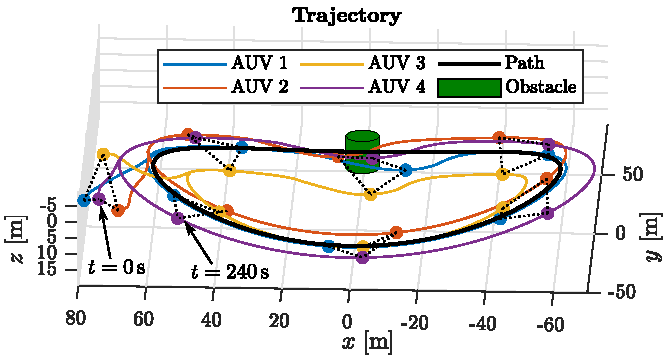
\includegraphics[width=0.75\textwidth]{figures/distr_NSB/sim_trajectory.pdf}
    \vspace{-4mm}
    \caption{The 3D trajectory of the AUVs. The markers represent the AUVs at times $t = 0, 40, \ldots, 240$ seconds. The dotted lines represent the communications graph.}
    \label{fig:distr_NSB_sim_trajectory}
\end{figure}


The purpose of this simulation is to demonstrate that the path-following, formation-keeping, and consensus errors of the continuous-time scheme converge to zero.
To satisfy the assumptions of Lemma~\ref{lemma2}, the consensus gain $c_s$ must be greater than $\frac{2 U_d k_s}{\lambda_2} = 0.65$. We choose $c_s = c_p = 1$.
To test the obstacle avoidance scheme, we place a static obstacle at $\mat{p}_o = \inlinevector{0, 40}$ with radius $r_o = \SI{5}{\meter}$.
The minimum cone $\alpha_{\min}$ is set to $2$ degrees, and the formation radius update gain is $k_r = 0.1$.

The results are shown in \figref{fig:distr_NSB_simulation}.
\figref{fig:distr_NSB_sim_trajectory} shows the 3D trajectory of the \glspl{auv}. We can see that the \glspl{auv} converge to their desired formation while avoiding the obstacle represented by the green cylinder.
\figref{fig:distr_NSB_sim_errors} shows the path-following and formation-keeping errors. Initially, these errors exponentially converge to zero. When the obstacle avoidance scheme is activated, the path-following errors start diverging, as the \gls{los} velocity enters the collision cone. After the vehicles successfully avoid the obstacle, the errors again converge exponentially to zero.
\figref{fig:distr_NSB_sim_distance} shows the distance between the \glspl{auv} and the obstacle. We can see that the distance is always greater than $r_o$.
Figs.~\ref{fig:distr_NSB_sim_barycenter}, \ref{fig:distr_NSB_sim_parameter}, and \ref{fig:distr_NSB_sim_radius} show the errors of the consensus variables. These plots are in a logarithmic scale to demonstrate the exponential rate of convergence. Initially, the logarithmic error is clearly bounded by a decreasing straight line, demonstrating the exponential convergence. The norm of the error decreases by a factor of 10 approximately every 25 seconds. When obstacle avoidance is active, the errors start diverging but remain bounded. After avoiding the obstacle, the errors continue to decrease exponentially, but eventually, the convergence stagnates. We cannot expect that the errors continue to fall indefinitely due to numerical innacuracies, that come mostly from two sources: the inaccuracies in floating-point arithmetics and the tolerances of the ODE solver.

Note that although Section~\ref{sec:distr_NSB_closed_loop} presents stability proof for a simplified case of straight-line paths and vehicles with single-integrator dynamics, the simulation results show stability for curved paths and more complex vehicle models.

\subsection{Event-Triggered Consensus}

In this section, we test the event-triggered scheme proposed in Section~\ref{sec:distr_NSB_event_triggered}.
We choose the mixing gains $a_p = a_s = 0.4$, and the penalty gains: $b_p = 10^{-4}, b_s = 4$.

We compare our algorithm with an event-triggered cooperative path following algorithm proposed in \cite{praveen_cooperative_2018}.
In this algorithm, each vehicle follows its own desired path given by $\mat{p}_{d,i}(s) = \mat{p}_p(s) + \mat{R}_p(s) \mat{p}_{f, i}^f$.
Coordination is then achieved by running a consensus scheme on the path parameter.

The comparison was done using a Monte Carlo simulation.
We performed ten thousand simulations with randomly selected initial conditions and communication delays.
The initial positions of the \glspl{auv} ranged from $\inlinevector{60,-40,0}$ to $\inlinevector{140,40,15}$.
The initial orientations were specified in Euler angles, with a zero roll angle, a pitch angle from $-\frac{\pi}{8}$ to $\frac{\pi}{8}$, and a yaw angle from $0$ to $\pi$.
The initial linear velocities ranged from $\inlinevector{0.5, -0.2, -0.1}$ to $\inlinevector{1.5, 0.2, 0.1}$, and the initial angular velocities were zero.
The communication delays ranged from $0$ to $5$ seconds.

\begin{figure}[t]
    \centering
    \begin{subfigure}{0.475\textwidth}
        % This file was created by matlab2tikz.
%
%The latest updates can be retrieved from
%  http://www.mathworks.com/matlabcentral/fileexchange/22022-matlab2tikz-matlab2tikz
%where you can also make suggestions and rate matlab2tikz.
%
\definecolor{mycolor1}{rgb}{0.00000,0.44700,0.74100}%
\definecolor{mycolor2}{rgb}{0.85000,0.32500,0.09800}%
%
\begin{tikzpicture}

\begin{axis}[%
width=0.7\textwidth,
height=20mm,
scale only axis,
xmin=0,
xmax=400,
xlabel style={font=\color{white!15!black}, yshift=1.7mm},
xlabel={Time [s]},
ymin=1e-7,
ymax=1,
ymode=log,
ylabel style={font=\color{white!15!black}, yshift=-2mm},
ylabel={$|\tilde{s}_i|$ [m]},
axis background/.style={fill=white},
axis x line*=bottom,
axis y line*=left,
xmajorgrids,
ymajorgrids,
title style={font=\bfseries, yshift=-2mm},
title={Path parameter error},
]

\addplot[area legend, dashed, draw=mycolor1, fill=mycolor1, fill opacity=0.15, forget plot]
table[] {comparison_parameter-1.tsv}--cycle;
\addplot [color=mycolor1, line width=0.8pt]
  table[]{comparison_parameter-2.tsv};
%\addlegendentry{NSB}

\addplot[area legend, dashed, draw=mycolor2, fill=mycolor2, fill opacity=0.15, forget plot]
table[] {comparison_parameter-3.tsv}--cycle;
\addplot [color=mycolor2, line width=0.8pt]
  table[]{comparison_parameter-4.tsv};
%\addlegendentry{CPF}
\end{axis}

\end{tikzpicture}%
        \label{fig:distr_NSB_comparison_parameter}
        \vspace{-8.5mm}
    \end{subfigure}
    \begin{subfigure}{0.475\textwidth}
        % This file was created by matlab2tikz.
%
%The latest updates can be retrieved from
%  http://www.mathworks.com/matlabcentral/fileexchange/22022-matlab2tikz-matlab2tikz
%where you can also make suggestions and rate matlab2tikz.
%
\definecolor{mycolor1}{rgb}{0.00000,0.44700,0.74100}%
\definecolor{mycolor2}{rgb}{0.85000,0.32500,0.09800}%
%
\begin{tikzpicture}

\begin{axis}[%
width=0.7\textwidth,
height=20mm,
scale only axis,
xmin=0,
xmax=400,
xlabel style={font=\color{white!15!black}, yshift=1.7mm},
xlabel={Time [s]},
ymin=0.01,
ymax=100,
ymode=log,
ylabel style={font=\color{white!15!black}, yshift=-2mm},
ylabel={$\|\mat{p}_b^p\|$ [m]},
axis background/.style={fill=white},
axis x line*=bottom,
axis y line*=left,
xmajorgrids,
ymajorgrids,
legend style={/tikz/column 2/.style={column sep=5pt,}, font=\small, at={(0.98,0.95)}, anchor=north east},
legend columns=2,
title style={font=\bfseries, yshift=-2mm},
title={Path-following error},
]

\addplot[area legend, dashed, draw=mycolor1, fill=mycolor1, fill opacity=0.15, forget plot]
table[] {comparison_barycenter-1.tsv}--cycle;
\addplot [color=mycolor1, line width=0.8pt]
  table[]{comparison_barycenter-2.tsv};
\addlegendentry{NSB}

\addplot[area legend, dashed, draw=mycolor2, fill=mycolor2, fill opacity=0.15, forget plot]
table[] {comparison_barycenter-3.tsv}--cycle;
\addplot [color=mycolor2, line width=0.8pt]
  table[]{comparison_barycenter-4.tsv};
\addlegendentry{CPF}
\end{axis}

\end{tikzpicture}%
        \label{fig:distr_NSB_comparison_barycenter}
        \vspace{-8.5mm}
    \end{subfigure}
    \caption{Comparison between the proposed event-triggered distributed NSB algorithm and the cooperative path-following algorithm proposed in \cite{praveen_cooperative_2018}. The full lines represent the median, the colored areas represent the smallest and largest recorded value.}
    \label{fig:distr_NSB_comparison}
\end{figure}


\figref{fig:distr_NSB_comparison} shows the absolute value of the path parameter error and the norm of the path-following error.
Both errors are plotted in a logarithmic scale.
In terms of path parameter errors, both algorithms perform similarly.
In terms of path-following errors, the distributed \gls{nsb} algorithm is marginally better.

The communication requirements of the two algorithms are summarized in Table~\ref{tab:comparison}.
This table shows the minimum, maximum, and median of the period in-between transmissions ($\tau_t$), and the total number of transmissions in one simulation ($N_t$).
Here, we can see that distributed \gls{nsb} performs considerably better in comparison to the cooperative path following method, with longer periods in-between transmissions and a lower number of transmissions.

However, it is worth mentioning that the packets transmitted by the cooperative path following method are smaller than the \gls{nsb} packets.
Indeed, in the scheme proposed in \cite{praveen_cooperative_2018}, the \glspl{auv} only need to transmit the path parameter and its derivative.
In contrast, the \gls{nsb} packet consists of the estimates of path parameter, barycenter, radius of formation, and formation-keeping error.
In this context, the two algorithms present a trade-off between packet size and communication periods.

\begin{table}[htb]
    \centering
    \caption{Comparison of communication requirements.}
    \label{tab:comparison}
    \begin{tabular}[t]{c|c|c|c|c}
        \textbf{Method}                                & \textbf{Quantity} & \textbf{Minimum} & \textbf{Median} & \textbf{Maximum} \\ \hline
        \multirow{2}{20mm}{Distributed NSB}            & $\tau_t$          & 2.00             & 8.50            & 275.30  \\
                                                       & $N_t$             & 125              & 187             & 253     \\ \hline
        \multirow{2}{20mm}{Coordinated path following} & $\tau_t$          & 0.10             & 2.15            & 138.65  \\
                                                       & $N_t$             & 196              & 548             & 1064 
    \end{tabular}
\end{table}


\section{Experiments}
\label{sec:distr_NSB_experiments}
In this section, we present the results of field experiments we designed and executed to verify the effectiveness of the event-triggered distributed \gls{nsb} algorithm proposed in Section~\ref{sec:distr_NSB_event_triggered}.
The experiments were conducted in the fjord of Trondheim, Norway, near the Trondheim Biological Station, using two \glspl{lauv} as in \figref{fig:distr_NSB_LAUV}.

\begin{figure}[b]
    \centering
    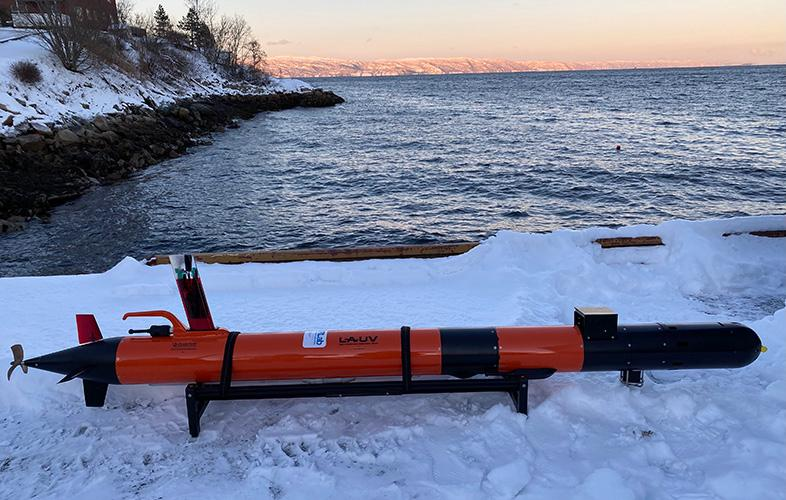
\includegraphics[width = 0.6\columnwidth]{figures/distr_NSB/LAUV-Roald}
    \caption{Photo of one of the two \glspl{lauv} used in the reported field experiments, courtesy of \url{www.ntnu.edu/aur-lab/}.}
    \label{fig:distr_NSB_LAUV}
\end{figure}

To guarantee stable communications and accurate navigation, the vehicles were operating at the surface and communicating over WiFi.
The algorithm was implemented in C++, using the Unified Navigation Environment (DUNE) \cite{dune}.

The algorithm was tested in two scenarios: a \emph{nominal} scenario, \emph{i.e.,} formation path following without any obstacles, and a scenario with a static obstacle.
In both scenarios, the barycenter of the \glspl{auv} should follow the elliptic path
\begin{align}
    \mat{p}_p(s) &= \inlinevector{a \cos(s), b \sin(s), 0},& 
    a &= \SI{100}{\meter},& 
    b &= \SI{80}{\meter},
\end{align}
in the formation defined by
\begin{align}
    \mat{p}_{f, 1}^f &= \inlinevector{0, -25, 0}, &
    \mat{p}_{f, 2}^f &= \inlinevector{0, 25, 0}.
\end{align}
The reason for choosing a larger path and formation, compared to the simulations in Section~\ref{sec:distr_NSB_simulations}, was to reduce the risk of the \glspl{auv} colliding.
The obstacle was placed at $\mat{p}_o = \inlinevector{0, 80}$.
The remaining parameters were identical to the simulations.

\subsection{Nominal Scenario}
\begin{figure}[p]
    \begin{minipage}{0.48\textwidth}
        \begin{subfigure}{\textwidth}
            % This file was created by matlab2tikz.
%
%The latest updates can be retrieved from
%  http://www.mathworks.com/matlabcentral/fileexchange/22022-matlab2tikz-matlab2tikz
%where you can also make suggestions and rate matlab2tikz.
%
\definecolor{mycolor1}{rgb}{0.00000,0.44700,0.74100}%
\definecolor{mycolor2}{rgb}{0.85000,0.32500,0.09800}%
%
\begin{tikzpicture}

\begin{axis}[%
width=0.85\textwidth,
height=75mm,
xmin=10.3555,
xmax=10.36,
xtick={10.358333},
xticklabels={$10^{\circ}21.50'$},
tick label style={font=\small},
xlabel style={font=\color{white!15!black},yshift=1.5mm},
xlabel={Longitude},
ymin=63.43465,
ymax=63.4371,
ytick={63.4350,63.4358,63.4367},
yticklabels={$63^{\circ}26.10'$, $63^{\circ}26.15'$, $63^{\circ}26.20'$},
xmajorgrids,
ymajorgrids,
ylabel style={font=\color{white!15!black}},
ylabel={Latitude},
axis background/.style={fill=white},
title style={font=\bfseries,yshift=-2.25mm},
title={Trajectory},
%legend style={/tikz/column 2/.style={column sep=2pt,}, font=\small, at={(1.12,1.08)}, anchor=north east},
%legend columns=1
]
\addplot [color=mycolor1, line width=0.8pt]
  table[]{experiment_nominal_trajectory-1.tsv};
%\addlegendentry{AUV 1}

\addplot[only marks, mark=*, mark options={}, mark size=2.5000pt, draw=mycolor1, fill=mycolor1, forget plot] table[]{experiment_nominal_trajectory-2.tsv};
\addplot [color=mycolor2, line width=0.8pt]
  table[]{experiment_nominal_trajectory-3.tsv};
%\addlegendentry{AUV 2}

\addplot[only marks, mark=*, mark options={}, mark size=2.5000pt, draw=mycolor2, fill=mycolor2, forget plot] table[]{experiment_nominal_trajectory-4.tsv};
\addplot [color=black, line width=0.8pt]
  table[]{experiment_nominal_trajectory-5.tsv};
%\addlegendentry{Path}

\addplot[only marks, mark=square*, mark options={}, mark size=1.8607pt, draw=black, fill=black, forget plot] table[]{experiment_nominal_trajectory-6.tsv};
\end{axis}
\end{tikzpicture}%
            \vspace{-3mm}
            \caption{The trajectory of the AUVs. The markers represent the AUVs at times $t = 0, 60, \ldots, 420$ seconds.}
            \label{fig:distr_NSB_experiment_nominal_trajectory}
        \end{subfigure}

        %\vspace{-4mm}

        \begin{subfigure}{\textwidth}
            % This file was created by matlab2tikz.
%
%The latest updates can be retrieved from
%  http://www.mathworks.com/matlabcentral/fileexchange/22022-matlab2tikz-matlab2tikz
%where you can also make suggestions and rate matlab2tikz.
%
\definecolor{mycolor1}{rgb}{0.00000,0.44700,0.74100}%
\definecolor{mycolor2}{rgb}{0.85000,0.32500,0.09800}%
\definecolor{mycolor3}{rgb}{0.92900,0.69400,0.12500}%
\definecolor{mycolor4}{rgb}{0.49400,0.18400,0.55600}%
%
\begin{tikzpicture}

\begin{axis}[%
width=0.8\textwidth,
height=18mm,
scale only axis,
xmin=0,
xmax=450,
xlabel style={font=\color{white!15!black},yshift=1.5mm},
xlabel={Time [s]},
ymin=-0.0004,
ymax=0.0004,
ylabel style={font=\color{white!15!black},yshift=-1.5mm},
ylabel={$\tilde{s}_i$ [--]},
xmajorgrids,
ymajorgrids,
axis background/.style={fill=white},
title style={font=\bfseries},
title={Path parameter errors},
legend style={/tikz/column 2/.style={column sep=2pt,}, font=\small},
legend columns=2
]
\addplot [color=mycolor1, line width=0.8pt]
  table[]{experiment_nominal_parameter-1.tsv};
\addlegendentry{AUV 1}

\addplot [color=mycolor2, line width=0.8pt]
  table[]{experiment_nominal_parameter-2.tsv};
\addlegendentry{AUV 2}

\addplot[only marks, mark=x, mark options={}, mark size=3.000pt, draw=mycolor1, forget plot] table[]{experiment_nominal_parameter-3.tsv};
\addplot[only marks, mark=x, mark options={}, mark size=3.000pt, draw=mycolor2, forget plot] table[]{experiment_nominal_parameter-4.tsv};
\end{axis}

\end{tikzpicture}%
            \vspace{-7mm}
            \caption{The path parameter errors. The markers represent transmissions.}
            \label{fig:distr_NSB_experiment_nominal_parameter}
        \end{subfigure}
    \end{minipage}
    \hspace{\fill}
    \begin{minipage}{0.48\textwidth}

        \hspace*{\fill}
        \begin{subfigure}{\textwidth}
            \hspace*{-5mm}
            % This file was created by matlab2tikz.
%
%The latest updates can be retrieved from
%  http://www.mathworks.com/matlabcentral/fileexchange/22022-matlab2tikz-matlab2tikz
%where you can also make suggestions and rate matlab2tikz.
%
\definecolor{mycolor1}{rgb}{0.00000,0.44700,0.74100}%
\definecolor{mycolor2}{rgb}{0.85000,0.32500,0.09800}%
%
\begin{tikzpicture}

\begin{axis}[%
width=0.8\textwidth,
height=18mm,
at={(0,27mm)},
scale only axis,
xmin=0,
xmax=450,
%xlabel style={font=\color{white!15!black},yshift=1.5mm},
%xlabel={Time [s]},
ymin=-30.2222476170977,
ymax=10,
ylabel style={font=\color{white!15!black},yshift=-1.5mm},
ylabel={$x$ [m]},
xmajorgrids,
ymajorgrids,
axis background/.style={fill=white},
title style={font=\bfseries,yshift=-2.5mm},
title={Formation path-following errors},
legend style={/tikz/column 2/.style={column sep=2pt,}, font=\small},
legend columns=3
]
\addplot [color=mycolor1, line width=0.8pt]
  table[]{experiment_nominal_errors-1.tsv};
%\addlegendentry{$\tilde{\sigma}_1$}

\addplot [color=mycolor2, line width=0.8pt]
  table[]{experiment_nominal_errors-2.tsv};
%\addlegendentry{$\tilde{\sigma}_2$}

\addplot [color=black, line width=0.8pt]
  table[]{experiment_nominal_errors-3.tsv};
%\addlegendentry{$\mat{p}_b^p$}

\end{axis}

\begin{axis}[%
width=0.55\textwidth,
height=8mm,
scale only axis,
at={(0.22\textwidth, 30mm)},
xmin=250,
xmax=450,
ymin=-2.2,
ymax=2.2,
axis background/.style={fill=white},
tick label style={font=\scriptsize},
xticklabel style={yshift=0.5mm},
yticklabel style={xshift=0.5mm},
xmajorgrids,
ymajorgrids,
]
\addplot [color=mycolor1, forget plot, line width=0.8pt]
  table[]{experiment_nominal_errors-4.tsv};
\addplot [color=mycolor2, forget plot, line width=0.8pt]
  table[]{experiment_nominal_errors-5.tsv};
\addplot [color=black, forget plot, line width=0.8pt]
  table[]{experiment_nominal_errors-6.tsv};
\end{axis}

\begin{axis}[%
width=0.8\textwidth,
height=19mm,
scale only axis,
at={(0,0)},
xmin=0,
xmax=450,
xlabel style={font=\color{white!15!black},yshift=1.5mm},
xlabel={Time [s]},
ymin=-12,
ymax=6,
ylabel style={font=\color{white!15!black},yshift=-2mm},
ylabel={$y$ [m]},
xmajorgrids,
ymajorgrids,
axis background/.style={fill=white},
legend style={/tikz/column 2/.style={column sep=2pt,}, font=\small, at={(0.98,1.25)}, anchor=north east},
legend columns=3
]
\addplot [color=mycolor1, line width=0.8pt]
  table[]{experiment_nominal_errors-7.tsv};
\addlegendentry{$\tilde{\bs{\sigma}}_1$}

\addplot [color=mycolor2, line width=0.8pt]
  table[]{experiment_nominal_errors-8.tsv};
\addlegendentry{$\tilde{\bs{\sigma}}_2$}

\addplot [color=black, line width=0.8pt]
  table[]{experiment_nominal_errors-9.tsv};
\addlegendentry{$\mat{p}_b^p$}

\end{axis}

\begin{axis}[%
width=0.55\textwidth,
height=8mm,
scale only axis,
at={(0.22\textwidth, 2.5mm)},
xmin=250,
xmax=450,
ymin=-1.8,
ymax=1.5,
axis background/.style={fill=white},
tick label style={font=\scriptsize},
xticklabel style={yshift=1mm},
yticklabel style={xshift=0.5mm},
xmajorgrids,
ymajorgrids,
]
\addplot [color=mycolor1, forget plot, line width=0.8pt]
  table[]{experiment_nominal_errors-10.tsv};
\addplot [color=mycolor2, forget plot, line width=0.8pt]
  table[]{experiment_nominal_errors-11.tsv};
\addplot [color=black, forget plot, line width=0.8pt]
  table[]{experiment_nominal_errors-12.tsv};
\end{axis}
\end{tikzpicture}%

            \vspace{-7mm}
            \caption{The path-following and formation-keeping errors.}
            \label{fig:distr_NSB_experiment_nominal_errors}
        \end{subfigure}

        %\vspace{-4mm}

        \hspace*{\fill}
        \begin{subfigure}{\textwidth}
            \hspace*{-5mm}
            % This file was created by matlab2tikz.
%
%The latest updates can be retrieved from
%  http://www.mathworks.com/matlabcentral/fileexchange/22022-matlab2tikz-matlab2tikz
%where you can also make suggestions and rate matlab2tikz.
%
\definecolor{mycolor1}{rgb}{0.00000,0.44700,0.74100}%
\definecolor{mycolor2}{rgb}{0.85000,0.32500,0.09800}%
%
\begin{tikzpicture}

\begin{axis}[%
width=0.8\textwidth,
height=15mm,
scale only axis,
at={(0,23mm)},
xmin=0,
xmax=450,
%xlabel style={font=\color{white!15!black},yshift=1.5mm},
%xlabel={Time [s]},
ymin=-2,
ymax=2,
ylabel style={font=\color{white!15!black},yshift=-1.5mm},
ylabel={$x$ [m]},
xmajorgrids,
ymajorgrids,
axis background/.style={fill=white},
title style={font=\bfseries,yshift=-2.5mm},
title={Barycenter estimate errors},
legend style={/tikz/column 2/.style={column sep=2pt,}, font=\small, at={(0.98,0.01)}, anchor=south east},
]
\addplot [color=mycolor1, line width=0.8pt]
  table[]{experiment_nominal_barycenter-1.tsv};
%\addlegendentry{AUV 1}

\addplot [color=mycolor2, line width=1pt, dashed]
  table[]{experiment_nominal_barycenter-2.tsv};
%\addlegendentry{AUV 2}

\end{axis}

\begin{axis}[%
width=0.8\textwidth,
height=15mm,
scale only axis,
at={(0,0)},
xmin=0,
xmax=450,
xlabel style={font=\color{white!15!black},yshift=1.5mm},
xlabel={Time [s]},
ymin=-2,
ymax=3,
ylabel style={font=\color{white!15!black},yshift=-1.5mm},
ylabel={$y$ [m]},
xmajorgrids,
ymajorgrids,
axis background/.style={fill=white},
legend style={/tikz/column 2/.style={column sep=2pt,}, font=\small, at={(0.98,1)}, anchor=north east},
legend columns=2
]
\addplot [color=mycolor1, line width=0.8pt]
  table[]{experiment_nominal_barycenter-3.tsv};
\addlegendentry{AUV 1}

\addplot [color=mycolor2, line width=1pt, dashed]
  table[]{experiment_nominal_barycenter-4.tsv};
\addlegendentry{AUV 2}

\end{axis}

\end{tikzpicture}%
            \vspace{-7mm}
            \caption{The $x$- and $y$-components of barycenter estimate errors.}
            \label{fig:distr_NSB_experiment_nominal_barycenter}
        \end{subfigure}
    \end{minipage}

    \caption{Results of a nominal experiment.}
    \label{fig:distr_NSB_experiment_nominal}
\end{figure}


The results are shown in \figref{fig:distr_NSB_experiment_nominal}.
\figref{fig:distr_NSB_experiment_nominal_trajectory} shows the trajectories of the \glspl{auv}, as estimated by their onboard navigation system.
The disturbances in the trajectories are caused by two factors: the sea loads (waves, currents, and wind), and the errors of the navigation system.
However, the exponential stability of the \gls{nsb} algorithm given by Theorem~\ref{thm_distr_NSB} provides some robustness towards these disturbances, \emph{c.f.,} \cite[Lemma 9.2]{khalil_nonlinear_2002}.
\figref{fig:distr_NSB_experiment_nominal_parameter} shows the path parameter errors and the event-triggered communications.
Initially, the vehicles need to communicate frequently, approximately every five seconds, because the barycenter estimates differ (as seen in \figref{fig:distr_NSB_experiment_nominal_barycenter}).
During this transient period, the path parameter estimates initially diverge before finally converging.
After convergence, the communication period increases to over 100 seconds.
Note that the barycenter estimate errors in \figref{fig:distr_NSB_experiment_nominal_barycenter} converge to a common value but not to zero.
This behavior is caused by the aforementioned disturbances acting on the vehicles.
\figref{fig:distr_NSB_experiment_nominal_errors} shows the formation-keeping and path-following errors.
Due to the disturbances and event-triggered communications, these errors do not converge to zero but rather to a small area near zero.

\subsection{Scenario with a Static Obstacle}
\begin{figure}[p]
    \begin{minipage}{0.48\textwidth}
        \begin{subfigure}{\textwidth}
            % This file was created by matlab2tikz.
%
%The latest updates can be retrieved from
%  http://www.mathworks.com/matlabcentral/fileexchange/22022-matlab2tikz-matlab2tikz
%where you can also make suggestions and rate matlab2tikz.
%
\definecolor{mycolor1}{rgb}{0.00000,0.44700,0.74100}%
\definecolor{mycolor2}{rgb}{0.85000,0.32500,0.09800}%
\definecolor{dkgreen}{rgb}{0,0.60000,0}
%
\begin{tikzpicture}

\begin{axis}[%
width=0.85\textwidth,
height=75mm,
xmin=10.3555,
xmax=10.36,
xtick={10.358333},
xticklabels={$10^{\circ}21.50'$},
tick label style={font=\small},
xlabel style={font=\color{white!15!black},yshift=1.5mm},
xlabel={Longitude},
ymin=63.43465,
ymax=63.4371,
ytick={63.4350,63.4358,63.4367},
yticklabels={$63^{\circ}26.10'$, $63^{\circ}26.15'$, $63^{\circ}26.20'$},
xmajorgrids,
ymajorgrids,
ylabel style={font=\color{white!15!black}},
ylabel={Latitude},
axis background/.style={fill=white},
title style={font=\bfseries,yshift=-2.25mm},
title={Trajectory},
%legend style={/tikz/column 2/.style={column sep=2pt,}, font=\small, at={(1.3,1.05)}, anchor=north east},
%legend columns=1
]
\addplot [color=mycolor1, line width=0.8pt]
  table[]{experiment_obstacle_trajectory-1.tsv};
%\addlegendentry{AUV 1}

\addplot[only marks, mark=*, mark options={}, mark size=2.5000pt, draw=mycolor1, fill=mycolor1, forget plot] table[]{experiment_obstacle_trajectory-2.tsv};
\addplot [color=mycolor2, line width=0.8pt]
  table[]{experiment_obstacle_trajectory-3.tsv};
%\addlegendentry{AUV 2}

\addplot[only marks, mark=*, mark options={}, mark size=2.5000pt, draw=mycolor2, fill=mycolor2, forget plot] table[]{experiment_obstacle_trajectory-4.tsv};
\addplot [color=black, line width=0.8pt]
  table[]{experiment_obstacle_trajectory-5.tsv};
%\addlegendentry{Path}

\addplot[only marks, mark=square*, mark options={}, mark size=1.8607pt, draw=black, fill=black, forget plot] table[]{experiment_obstacle_trajectory-6.tsv};

\addplot[area legend, draw=none, fill=dkgreen]
table[] {experiment_obstacle_trajectory-7.tsv}--cycle;
%\addlegendentry{Obstacle}

\end{axis}
\end{tikzpicture}%
            \vspace{-2mm}
            \caption{The trajectory of the AUVs. The markers represent the AUVs at times $t = 0, 60, \ldots, 420$ seconds.}
            \label{fig:distr_NSB_experiment_obstacle_trajectory}
        \end{subfigure}

        %\vspace{-4mm}

        \hspace*{\fill}
        \begin{subfigure}{\textwidth}
            \hspace*{-3mm}
            % This file was created by matlab2tikz.
%
%The latest updates can be retrieved from
%  http://www.mathworks.com/matlabcentral/fileexchange/22022-matlab2tikz-matlab2tikz
%where you can also make suggestions and rate matlab2tikz.
%
\definecolor{mycolor1}{rgb}{0.00000,0.44700,0.74100}%
\definecolor{mycolor2}{rgb}{0.85000,0.32500,0.09800}%
%
\begin{tikzpicture}

\begin{axis}[%
width=0.8\textwidth,
height=18mm,
at={(0,27mm)},
scale only axis,
xmin=0,
xmax=450,
%xlabel style={font=\color{white!15!black},yshift=1.5mm},
%xlabel={$t$ [s]},
ymin=-30.2222476170977,
ymax=10,
ylabel style={font=\color{white!15!black},yshift=-1.5mm},
ylabel={$x$ [m]},
xmajorgrids,
ymajorgrids,
axis background/.style={fill=white},
title style={font=\bfseries,yshift=-2.5mm,xshift=-8mm},
title={Formation path-following errors},
legend style={/tikz/column 2/.style={column sep=2pt,}, font=\small},
legend columns=3
]
\addplot[area legend, dashed, draw=black, fill=green, fill opacity=0.15, forget plot]
table[] {experiment_obstacle_errors-area-1.tsv}--cycle;

\addplot [color=mycolor1, line width=0.8pt]
  table[]{experiment_obstacle_errors-1.tsv};
%\addlegendentry{$\tilde{\sigma}_1$}

\addplot [color=mycolor2, line width=0.8pt]
  table[]{experiment_obstacle_errors-2.tsv};
%\addlegendentry{$\tilde{\sigma}_2$}

\addplot [color=black, line width=0.8pt]
  table[]{experiment_obstacle_errors-3.tsv};
%\addlegendentry{$\mat{p}_b^p$}

\end{axis}

\begin{axis}[%
width=0.45\textwidth,
height=8mm,
scale only axis,
at={(0.32\textwidth, 30mm)},
xmin=250,
xmax=450,
ymin=-2,
ymax=2,
axis background/.style={fill=white},
tick label style={font=\scriptsize},
xticklabel style={yshift=0.5mm},
yticklabel style={xshift=0.5mm},
xmajorgrids,
ymajorgrids,
]
\addplot [color=mycolor1, forget plot, line width=0.8pt]
  table[]{experiment_obstacle_errors-4.tsv};
\addplot [color=mycolor2, forget plot, line width=0.8pt]
  table[]{experiment_obstacle_errors-5.tsv};
\addplot [color=black, forget plot, line width=0.8pt]
  table[]{experiment_obstacle_errors-6.tsv};
\end{axis}

\begin{axis}[%
width=0.8\textwidth,
height=19mm,
scale only axis,
at={(0,0)},
xmin=0,
xmax=450,
xlabel style={font=\color{white!15!black},yshift=1.5mm},
xlabel={$t$ [s]},
ymin=-15,
ymax=31,
ytick={-10,0,10,20,30},
ylabel style={font=\color{white!15!black},yshift=-2mm},
ylabel={$y$ [m]},
xmajorgrids,
ymajorgrids,
axis background/.style={fill=white},
legend style={/tikz/column 2/.style={column sep=2pt,}, font=\small, at={(0.98,-0.05)}, anchor=south east},
legend columns=3
]
\addplot[area legend, dashed, draw=black, fill=green, fill opacity=0.15, forget plot]
table[] {experiment_obstacle_errors-area-2.tsv}--cycle;

\addplot [color=mycolor1, line width=0.8pt]
  table[]{experiment_obstacle_errors-7.tsv};
\addlegendentry{$\tilde{\bs{\sigma}}_1$}

\addplot [color=mycolor2, line width=0.8pt]
  table[]{experiment_obstacle_errors-8.tsv};
\addlegendentry{$\tilde{\bs{\sigma}}_2$}

\addplot [color=black, line width=0.8pt]
  table[]{experiment_obstacle_errors-9.tsv};
\addlegendentry{$\mat{p}_b^p$}

\end{axis}

\begin{axis}[%
width=0.45\textwidth,
height=8mm,
scale only axis,
at={(0.32\textwidth, 10mm)},
xmin=250,
xmax=450,
ymin=-1.5,
ymax=1.2,
axis background/.style={fill=white},
tick label style={font=\scriptsize},
xticklabel style={yshift=1mm},
yticklabel style={xshift=0.5mm},
xmajorgrids,
ymajorgrids,
]
\addplot [color=mycolor1, forget plot, line width=0.8pt]
  table[]{experiment_obstacle_errors-10.tsv};
\addplot [color=mycolor2, forget plot, line width=0.8pt]
  table[]{experiment_obstacle_errors-11.tsv};
\addplot [color=black, forget plot, line width=0.8pt]
  table[]{experiment_obstacle_errors-12.tsv};
\end{axis}
\end{tikzpicture}%

            \vspace{-3mm}
            \caption{The path-following and formation-keeping errors. The green area represents the time when obstacle avoidance is active.}
            \label{fig:distr_NSB_experiment_obstacle_errors}
        \end{subfigure}
    \end{minipage}
    \hspace{\fill}
    \begin{minipage}{0.48\textwidth}

        \hspace*{-1mm}
        \begin{subfigure}{\textwidth}
            \hspace*{-3mm}
            % This file was created by matlab2tikz.
%
%The latest updates can be retrieved from
%  http://www.mathworks.com/matlabcentral/fileexchange/22022-matlab2tikz-matlab2tikz
%where you can also make suggestions and rate matlab2tikz.
%
\definecolor{mycolor1}{rgb}{0.00000,0.44700,0.74100}%
\definecolor{mycolor2}{rgb}{0.85000,0.32500,0.09800}%
\definecolor{mycolor3}{rgb}{0.92900,0.69400,0.12500}%
\definecolor{mycolor4}{rgb}{0.49400,0.18400,0.55600}%
%
\begin{tikzpicture}

\begin{axis}[%
width=0.8\textwidth,
height=18mm,
scale only axis,
xmin=0,
xmax=450,
xlabel style={font=\color{white!15!black},yshift=1.5mm},
xlabel={$t$ [s]},
ymin=-0.0004,
ymax=0.0004,
ylabel style={font=\color{white!15!black},yshift=-1.5mm},
ylabel={$\tilde{s}_i$ [--]},
xmajorgrids,
ymajorgrids,
axis background/.style={fill=white},
title style={font=\bfseries},
title={Path parameter errors},
legend style={/tikz/column 2/.style={column sep=2pt,}, font=\small},
legend columns=2
]
\addplot [color=mycolor1, line width=0.8pt]
  table[]{experiment_obstacle_parameter-1.tsv};
\addlegendentry{AUV 1}

\addplot [color=mycolor2, line width=0.8pt]
  table[]{experiment_obstacle_parameter-2.tsv};
\addlegendentry{AUV 2}

\addplot[only marks, mark=x, mark options={}, mark size=3.000pt, draw=mycolor1, forget plot] table[]{experiment_obstacle_parameter-3.tsv};
\addplot[only marks, mark=x, mark options={}, mark size=3.000pt, draw=mycolor2, forget plot] table[]{experiment_obstacle_parameter-4.tsv};
\end{axis}

\end{tikzpicture}%
            \vspace{-3mm}
            \caption{The path parameter errors. The markers represent transmissions.}
            \label{fig:distr_NSB_experiment_obstacle_parameter}
        \end{subfigure}

        %\vspace{-4mm}

        \hspace*{-1mm}
        \begin{subfigure}{\textwidth}
            \hspace*{-3mm}
            % This file was created by matlab2tikz.
%
%The latest updates can be retrieved from
%  http://www.mathworks.com/matlabcentral/fileexchange/22022-matlab2tikz-matlab2tikz
%where you can also make suggestions and rate matlab2tikz.
%
\definecolor{mycolor1}{rgb}{0.00000,0.44700,0.74100}%
\definecolor{mycolor2}{rgb}{0.85000,0.32500,0.09800}%
%
\begin{tikzpicture}

\begin{axis}[%
width=0.8\textwidth,
height=15mm,
scale only axis,
at={(0,20mm)},
xmin=0,
xmax=450,
%xlabel style={font=\color{white!15!black},yshift=1.5mm},
%xlabel={$t$ [s]},
ymin=-1,
ymax=2,
ylabel style={font=\color{white!15!black},yshift=-1.5mm},
ylabel={$x$ [m]},
xmajorgrids,
ymajorgrids,
axis background/.style={fill=white},
title style={font=\bfseries,yshift=-2.5mm},
title={Barycenter estimate errors},
legend style={/tikz/column 2/.style={column sep=2pt,}, font=\small, at={(0.98,0.01)}, anchor=south east},
]
\addplot [color=mycolor1, line width=0.8pt]
  table[]{experiment_obstacle_barycenter-1.tsv};
%\addlegendentry{AUV 1}

\addplot [color=mycolor2, line width=1pt, dashed]
  table[]{experiment_obstacle_barycenter-2.tsv};
%\addlegendentry{AUV 2}

\end{axis}

\begin{axis}[%
width=0.8\textwidth,
height=15mm,
scale only axis,
at={(0,0)},
xmin=0,
xmax=450,
xlabel style={font=\color{white!15!black},yshift=1.5mm},
xlabel={$t$ [s]},
ymin=-4,
ymax=1,
ylabel style={font=\color{white!15!black},yshift=-1.5mm},
ylabel={$y$ [m]},
xmajorgrids,
ymajorgrids,
axis background/.style={fill=white},
legend style={/tikz/column 2/.style={column sep=2pt,}, font=\small, at={(0.98,0.02)}, anchor=south east},
legend columns=2
]
\addplot [color=mycolor1, line width=0.8pt]
  table[]{experiment_obstacle_barycenter-3.tsv};
\addlegendentry{AUV 1}

\addplot [color=mycolor2, line width=1pt, dashed]
  table[]{experiment_obstacle_barycenter-4.tsv};
\addlegendentry{AUV 2}

\end{axis}

\end{tikzpicture}%
            \vspace{-3mm}
            \caption{The $x$- and $y$-components of barycenter estimate errors.}
            \label{fig:distr_NSB_experiment_obstacle_barycenter}
        \end{subfigure}


        %\vspace{-4mm}

        \hspace*{-1mm}
        \begin{subfigure}{\textwidth}
            % This file was created by matlab2tikz.
%
%The latest updates can be retrieved from
%  http://www.mathworks.com/matlabcentral/fileexchange/22022-matlab2tikz-matlab2tikz
%where you can also make suggestions and rate matlab2tikz.
%
\definecolor{mycolor1}{rgb}{0.00000,0.44700,0.74100}%
\definecolor{mycolor2}{rgb}{0.85000,0.32500,0.09800}%
%
\begin{tikzpicture}

\begin{axis}[%
width=0.8\textwidth,
height=16mm,
scale only axis,
xmin=0,
xmax=450,
xlabel style={font=\color{white!15!black},yshift=1.5mm},
xlabel={Time [s]},
ymin=1,
%ymax=60,
xmajorgrids,
ymajorgrids,
ymode=log,
ylabel style={font=\color{white!15!black},yshift=-1mm},
ylabel={Distance [m]},
axis background/.style={fill=white},
title style={font=\bfseries,yshift=-2.5mm},
title={Distance to obstacle},
%legend style={/tikz/column 2/.style={column sep=2pt,}, font=\small, at={(0.98,0.02)}, anchor=south east},
%legend columns=2
]
\addplot [color=mycolor1, line width=0.8pt]
  table[]{experiment_obstacle_distance-1.tsv};
%\addlegendentry{AUV 1}

\addplot [color=mycolor2, line width=0.8pt]
  table[]{experiment_obstacle_distance-2.tsv};
%\addlegendentry{AUV 2}

\addplot [color=black, dashed, line width=1pt]
  table[]{experiment_obstacle_distance-3.tsv};
%\addlegendentry{$r_o$}

\end{axis}

\end{tikzpicture}%
            \vspace{-3mm}
            \caption{The distance between the AUVs and the obstacle.}
            \label{fig:distr_NSB_experiment_obstacle_distance}
        \end{subfigure}

        %\vspace{-4mm}

        \hspace*{-1mm}
        \begin{subfigure}{\textwidth}
            % This file was created by matlab2tikz.
%
%The latest updates can be retrieved from
%  http://www.mathworks.com/matlabcentral/fileexchange/22022-matlab2tikz-matlab2tikz
%where you can also make suggestions and rate matlab2tikz.
%
\definecolor{mycolor1}{rgb}{0.00000,0.44700,0.74100}%
\definecolor{mycolor2}{rgb}{0.85000,0.32500,0.09800}%
%
\begin{tikzpicture}

\begin{axis}[%
width=0.8\textwidth,
height=16mm,
scale only axis,
xmin=0,
xmax=450,
xlabel style={font=\color{white!15!black},yshift=1.5mm},
xlabel={Time [s]},
ymin=-5,
ymax=10,
xmajorgrids,
ymajorgrids,
ylabel style={font=\color{white!15!black},yshift=-1mm},
ylabel={Error [m]},
axis background/.style={fill=white},
title style={font=\bfseries,yshift=-2.5mm},
title={Formation radius error},
legend style={/tikz/column 2/.style={column sep=2pt,}, font=\small, at={(0.98,0.98)}, anchor=north east},
legend columns=2
]
\addplot [color=mycolor1, line width=0.8pt]
  table[]{experiment_obstacle_radius-1.tsv};
\addlegendentry{AUV 1}

\addplot [color=mycolor2, line width=0.8pt]
  table[]{experiment_obstacle_radius-2.tsv};
\addlegendentry{AUV 2}

\end{axis}

\end{tikzpicture}%
            \vspace{-3mm}
            \caption{The error between the estimated and true formation radius.}
            \label{fig:distr_NSB_experiment_obstacle_radius}
        \end{subfigure}
    \end{minipage}

    \caption{Experiment with a static obstacle.}
    \label{fig:distr_NSB_experiment_obstacle}
\end{figure}


The results are shown in \figref{fig:distr_NSB_experiment_obstacle}.
In general, the results are similar to the nominal scenario, so we will only highlight the differences.
The path-following errors in \figref{fig:distr_NSB_experiment_obstacle_errors} diverge when obstacle avoidance is active.
As previously mentioned, this behavior is caused by the fact that the vehicles cannot stay on the desired path while avoiding the obstacle.
The estimate errors in Figs.~\ref{fig:distr_NSB_experiment_obstacle_parameter} and \ref{fig:distr_NSB_experiment_obstacle_barycenter} behave similarly to the nominal case.
As shown in \figref{fig:distr_NSB_experiment_obstacle_distance}, the distance between the \glspl{auv} and the obstacle is always greater than $r_o$.
\figref{fig:distr_NSB_experiment_obstacle_radius} shows the errors between the estimated and true formation radius.
Note that the formation radius errors are connected to the barycenter estimates.
A wrong barycenter estimate may lead to both overestimation and underestimation of the formation radius.
Despite these uncertainties, the \glspl{auv} still manage to perform all control goals safely.
